% -*- Mode:TeX -*-

%% The documentclass options along with the pagestyle can be used to generate
%% a technical report, a draft copy, or a regular thesis.  You may need to
%% re-specify the pagestyle after you \include  cover.tex.  For more
%% information, see the first few lines of mitthesis.cls. 

\documentclass[12pt]{mitthesis}
%\usepackage{lgrind}
%\usepackage{algorithmic}
%\usepackage{algorithm}
\usepackage{stmaryrd}
\usepackage{amsmath}
\usepackage{amsopn}
\usepackage{listings}
\usepackage{url}
\usepackage[nottoc]{tocbibind}
\pagestyle{plain}

\DeclareMathOperator{\find}{find}
\DeclareMathOperator{\conform}{conform}
\DeclareMathOperator{\subtype}{subtype}
\DeclareMathOperator{\typeof}{typeof}
\DeclareMathOperator{\eval}{eval}
\DeclareMathOperator{\interpret}{interpret}
\DeclareMathOperator{\incomplete}{incomplete}
%\DeclareMathOperator{\choose}{choose}
\DeclareMathOperator{\length}{length}
\DeclareMathOperator{\recall}{recall}
%\DeclareMathOperator{\empty}{empty}
\DeclareMathOperator{\tail}{tail}
\DeclareMathOperator{\Frame}{Frame}
\DeclareMathOperator{\extend}{extend}
\DeclareMathOperator{\super}{super}
\DeclareMathOperator{\p}{p}
\DeclareMathOperator{\last}{last}
\DeclareMathOperator{\typename}{typename}
\DeclareMathOperator{\intersect}{intersect}
\DeclareMathOperator{\formals}{formals}
\DeclareMathOperator{\superdecl}{super\_decl}

\lstdefinestyle{customjulia}{
  basicstyle=\small\ttfamily,
  escapeinside={~}{~},
}

%% This bit allows you to either specify only the files which you wish to
%% process, or `all' to process all files which you \include.
%% Krishna Sethuraman (1990).

%\typein [\files]{Enter file names to process, (chap1,chap2 ...), or `all' to
%process all files:}
%\def\all{all}
%\ifx\files\all \typeout{Including all files.} \else \typeout{Including only \files.} \includeonly{\files} \fi

\begin{document}

% -*-latex-*-
% $Log: cover.tex,v $
% Revision 1.7  2010/04/29 11:35:46  bryt
% changed department chair from Art Smith to Terry Orlando
% changed default copyright flag from author to MIT, left directions for changing it back
% 
% Revision 1.6  1999/10/21 14:49:31  boojum
% changed comment referring to documentstyle
%
% Revision 1.5  1999/10/21 14:39:04  boojum
% *** empty log message ***
%
% Revision 1.4  1997/04/18  17:54:10  othomas
% added page numbers on abstract and cover, and made 1 abstract
% page the default rather than 2.  (anne hunter tells me this
% is the new institute standard.)
%
% Revision 1.4  1997/04/18  17:54:10  othomas
% added page numbers on abstract and cover, and made 1 abstract
% page the default rather than 2.  (anne hunter tells me this
% is the new institute standard.)
%
% Revision 1.3  93/05/17  17:06:29  starflt
% Added acknowledgements section (suggested by tompalka)
% 
% Revision 1.2  92/04/22  13:13:13  epeisach
% Fixes for 1991 course 6 requirements
% Phrase "and to grant others the right to do so" has been added to 
% permission clause
% Second copy of abstract is not counted as separate pages so numbering works
% out
% 
% Revision 1.1  92/04/22  13:08:20  epeisach
\title{Abstraction in Technical Computing}

\author{Jeffrey Werner Bezanson}
\department{Department of Electrical Engineering and Computer Science}
% If the thesis is for two degrees simultaneously, list them both
% separated by \and like this:
% \degree{Doctor of Philosophy \and Master of Science}
\degree{Doctor of Philosophy}
\degreemonth{February}
\degreeyear{2015}
\thesisdate{January 9, 2015}

%% By default, the thesis will be copyrighted to MIT.  If you need to copyright
%% the thesis to yourself, just specify the `vi' documentclass option.  If for
%% some reason you want to exactly specify the copyright notice text, you can
%% use the \copyrightnoticetext command.  
%\copyrightnoticetext{\copyright IBM, 1990.  Do not open till Xmas.}

% If there is more than one supervisor, use the \supervisor command
% once for each.
\supervisor{Alan Edelman}{Professor}

% This is the department committee chairman, not the thesis committee
% chairman.  You should replace this with your Department's Committee
% Chairman.
\chairman{Leslie Kolodziejski}{Chairman, Department Committee on Graduate Students}

% Make the titlepage based on the above information.  If you need
% something special and can't use the standard form, you can specify
% the exact text of the titlepage yourself.  Put it in a titlepage
% environment and leave blank lines where you want vertical space.
% The spaces will be adjusted to fill the entire page.  The dotted
% lines for the signatures are made with the \signature command.
\maketitle

% The abstractpage environment sets up everything on the page except
% the text itself.  The title and other header material are put at the
% top of the page, and the supervisors are listed at the bottom.  A
% new page is begun both before and after.  Of course, an abstract may
% be more than one page itself.  If you need more control over the
% format of the page, you can use the abstract environment, which puts
% the word "Abstract" at the beginning and single spaces its text.

%% You can either \input (*not* \include) your abstract file, or you can put
%% the text of the abstract directly between the \begin{abstractpage} and
%% \end{abstractpage} commands.

% First copy: start a new page, and save the page number.
\newpage
% Uncomment the next line if you do NOT want a page number on your
% abstract and acknowledgments pages.
% \pagestyle{empty}
\setcounter{savepage}{\thepage}
\begin{abstractpage}
% $Log: abstract.tex,v $
% Revision 1.1  93/05/14  14:56:25  starflt
% Initial revision
% 
% Revision 1.1  90/05/04  10:41:01  lwvanels
% Initial revision
% 
%
%% The text of your abstract and nothing else (other than comments) goes here.
%% It will be single-spaced and the rest of the text that is supposed to go on
%% the abstract page will be generated by the abstractpage environment.  This
%% file should be \input (not \include 'd) from cover.tex.

Array-based programming environments are popular for scientific and
technical computing.
These systems consist of built-in function libraries paired with high-level
languages for interaction.
Although the libraries perform well, it is widely believed that scripting in these
languages is necessarily slow, and that only heroic feats of engineering can at
best partially ameliorate this problem.

This thesis argues that what is really needed is a more coherent
structure for this functionality.
To find one, we must ask what technical computing is really about.
This thesis suggests that this kind of programming is characterized by an emphasis on operator
complexity and code specialization, and that a language can be designed to
better fit these requirements.

The key idea is to integrate code \emph{selection} with code \emph{specialization},
using generic functions and data-flow type inference.
Systems like these can suffer from inefficient compilation, or from
uncertainty about what to specialize on.
We show that sufficiently powerful type-based dispatch addresses these problems.
The resulting language, Julia, achieves a Quine-style
``explication by elimination'' of many of the productive features
technical computing users expect.

% we show how this can be use to greatly simplify code for demanding
% scientific applications that require a mixture of binding times.

% thesis stmt: integrating code selection and specialization with
% type-based dynamic dispatch captures both the performance and
% productivity requirements of technical computing.

%For this role I propose an abstraction based on an extended version of
%generic functions.
%The novelty of this mechanism is that it is both flexible enough to describe
%the wide variety of behaviors users need in practice, while also providing
%enough information to a compiler to yield good performance.


% integration of selection and specialization

% making data-flow and specialization-based languages practical

% answers the question of what to specialize on

% applies Quine's ``explication through elimination'' to common features of T.C.

\end{abstractpage}

% Additional copy: start a new page, and reset the page number.  This way,
% the second copy of the abstract is not counted as separate pages.
% Uncomment the next 6 lines if you need two copies of the abstract
% page.
% \setcounter{page}{\thesavepage}
% \begin{abstractpage}
% % $Log: abstract.tex,v $
% Revision 1.1  93/05/14  14:56:25  starflt
% Initial revision
% 
% Revision 1.1  90/05/04  10:41:01  lwvanels
% Initial revision
% 
%
%% The text of your abstract and nothing else (other than comments) goes here.
%% It will be single-spaced and the rest of the text that is supposed to go on
%% the abstract page will be generated by the abstractpage environment.  This
%% file should be \input (not \include 'd) from cover.tex.

Array-based programming environments are popular for scientific and
technical computing.
These systems consist of built-in function libraries paired with high-level
languages for interaction.
Although the libraries perform well, it is widely believed that scripting in these
languages is necessarily slow, and that only heroic feats of engineering can at
best partially ameliorate this problem.

This thesis argues that what is really needed is a more coherent
structure for this functionality.
To find one, we must ask what technical computing is really about.
This thesis suggests that this kind of programming is characterized by an emphasis on operator
complexity and code specialization, and that a language can be designed to
better fit these requirements.

The key idea is to integrate code \emph{selection} with code \emph{specialization},
using generic functions and data-flow type inference.
Systems like these can suffer from inefficient compilation, or from
uncertainty about what to specialize on.
We show that sufficiently powerful type-based dispatch addresses these problems.
The resulting language, Julia, achieves a Quine-style
``explication by elimination'' of many of the productive features
technical computing users expect.

% we show how this can be use to greatly simplify code for demanding
% scientific applications that require a mixture of binding times.

% thesis stmt: integrating code selection and specialization with
% type-based dynamic dispatch captures both the performance and
% productivity requirements of technical computing.

%For this role I propose an abstraction based on an extended version of
%generic functions.
%The novelty of this mechanism is that it is both flexible enough to describe
%the wide variety of behaviors users need in practice, while also providing
%enough information to a compiler to yield good performance.


% integration of selection and specialization

% making data-flow and specialization-based languages practical

% answers the question of what to specialize on

% applies Quine's ``explication through elimination'' to common features of T.C.

% \end{abstractpage}

\newpage

\begin{singlespace}

\section*{Acknowledgments}

%thank Tim Holy for frequently and spontaneously writing explanations
%that I found myself wanting to copy and paste into this writeup.


\end{singlespace}

%%%%%%%%%%%%%%%%%%%%%%%%%%%%%%%%%%%%%%%%%%%%%%%%%%%%%%%%%%%%%%%%%%%%%%
% -*-latex-*-

\pagestyle{plain}
  % -*- Mode:TeX -*-
%% This file simply contains the commands that actually generate the table of
%% contents and lists of figures and tables.  You can omit any or all of
%% these files by simply taking out the appropriate command.  For more
%% information on these files, see appendix C.3.3 of the LaTeX manual. 
\renewcommand{\baselinestretch}{1.4}\normalsize
\tableofcontents
\renewcommand{\baselinestretch}{1.5}\normalsize
\newpage
\listoffigures
%\listofalgorithms
%\newpage
\listoftables
\newpage



\chapter{Introduction}

Scientific computing has evolved from being essentially the only kind of
computing that existed, to being a small part of how and why computers
are used.
Over this period of time, programming tools have advanced in terms of
the abstractions and generalizations they are capable of.

Science as a whole evolves through the incorporation of specialized bits
of knowledge into more powerful general theories.  
When we examine computer languages we see the parallel:  that
many special-purpose languages have been subsumed by languages that are more powerful and
general. 
How has this trend affected scientific computing?
The surprising answer is: not as much as we would like.
We see scientists and technical users generally either turning away
from the ``best'' new programming languages, or else pushing them
to their limits in unusual ways.

%% Much of the history of programming languages has been about increasing abstraction
%% and generalization. Today we take it for granted that a single suitably powerful
%% language could be used for nearly any programming task, were it not for pragmatic
%% factors beyond our control. Over time,
%% The field of technical computing --- programming for applied math and the
%% sciences --- is something of a holdout from this trend, with its own
%% purpose-built languages still dominating.
%% There are probably many reasons for this, including historical, social and
%% technical.

\begin{singlespace}
\begin{figure}
  \begin{center}
    \begin{tabular}{|llll|l|}\hline
      \multicolumn{4}{|c|}{Productivity} & Performance \\
      \hline
      Matlab  &  Maple &  Mathematica & SciPy & Fortress\\
      SciLab  &  IDL   &  R  & Octave         & Chapel \\
      S-PLUS  & SAS & J & APL                 & X10 \\
      Maxima & Mathcad & Axiom & Sage         & SAC \\
      Lush & Ch & LabView & O-Matrix          & ZPL \\
      PV-WAVE & Igor Pro & OriginLab & FreeMat &\\
      Yorick & GAUSS & MuPad & Genius &\\
      SciRuby & Ox & Stata & JLab &\\
      Magma & Euler & Rlab & Speakeasy &\\
      GDL & Nickle & gretl & ana &\\
      Torch7 & A+ & PDL & Nial & \\
      \hline
    \end{tabular}
  \end{center}
  \caption{
    49 technical computing languages classified as primarily designed for Productivity or Performance
  }
  \label{gangof40}
\end{figure}
\end{singlespace}

In fact, we have discovered at least \emph{49} programming languages
designed for technical computing since Fortran (figure~\ref{gangof40}).
This is a high number by any standard begging for  a reasonable hypothesis to
explain this high number.
We propose that users crave 
the flexibility to permit \emph{any} conceivable means of
describing computations.
Language design is then 
where you go when you need a lot
of this flexibility.
After all, language design is  associated with the highest level of abstraction.
The desire for scientists to rework their code  is not so surprising when one reflects on the tradition
of inventing new notation in mathematics and science.
%This certainly
%helps distinguish scientific programming from other application areas.

The need for language-level flexibility is corroborated by
the ways that the technical computing domain uses general purpose
languages.
Effective scientific libraries extensively employ
polymorphism, custom operators, and compile-time abstraction.
Code generation approaches (writing a program that writes the needed
program) are unusually common.
Most of these techniques are presently fairly difficult to use, and so
programmers working at this level give up the notational conveniences
of the purpose-built languages above.

%Yet it also demands the greatest ease-of-use.
%A good rule of thumb is that if you need to write a program that prints
%out code in language X, then language X is not powerful enough.

%pathologies arising from the language level are subtle
%not as immediate as ``this new matrix multiply is faster''


This thesis addresses the essential challenges created by
this state of affairs.
We argue that the situation   
can be improved considerably by
abstracting, with a new language.

%the essential challenges from the state
%f affairs we have described.
%Of course, a language is not the only thing the world of technical
%computing needs.
 Compiler \todo{see comment that follows}
techniques, library design, high-performance
computational kernels, new algorithms, and approaches to parallelism might
be as perhaps more important than language design.
However these sorts of technologies can usually be applied to multiple
languages, as has happened in the C and Fortran language families.
%, which have taken on many such extensions over the years.
So in our view languages targeting this space need to dig deeper,
at least temporarily forgetting about matrices and cache utilization,
and look for bigger patterns.
\todo[inline]{{\it Please consider if this is even more true: }\newline
Technical computing  can benefit from many technologies.
Some of these include compiler techniques, library design, high-performance
computational kernels, new algorithms, and new approaches to parallelism.
These sorts of technologies can usually be applied to multiple
languages, as has happened in the C and Fortran language families.
They do not by themselves insist that a new language be developed.
However in conjunction with a new language, these technologies can flourish.
Indeed, we believe that language design
has reached a level of importance that even (perhaps temporarily) supersedes
the traditional focus of cache utilization and the use of matrix operations.
}

In brief, our idea is to \emph{integrate code selection and specialization}.
The aforementioned flexibility requirement can be explained as
a sufficiently powerful means for \emph{selecting} which piece of code
to run. This notion subsumes method dispatch, function overloading,
and potentially even branches. When such mechanisms are used in
technical computing, there is nearly always a corresponding need to
\emph{specialize} code for specific cases to obtain performance.
Polymorphic languages sometimes support forms of specialization,
but often only through a designated mechanism (e.g. templates), or
deployed rather conservatively out of resource concerns.
We intend to show that an equilibrium point in the design
space can be found by combining selection and specialization
into a single dynamic multiple dispatch mechanism.
The specific design is identified via
subtyping theories and closure under data-flow operations.

%what does this system achieve?
%-

% why dynamic dispatch?
%% somewhat counter-intuitively, dynamic dispatch can be good for performance
%% since it permits invoking the most specialized possible method.
%% static overloading can lead to calling a sub-optimal case when multiple
%% overloads exist for the sake of performance.




%Extensive code specialization is a key feature of
%technical computing. ``what to specialize on'' has been an open problem.
%our types are a possible solution to this for two reasons:

%\begin{enumerate}
%\item you can tune the amount of information they contain
%\item everybody agrees to use them, which helps ensure that specializing on
%  the types will actually do something useful.
%\end{enumerate}

%the amazing thing about programming languages it that a better
%explanation can directly lead to better performance!)



%By \emph{selection} we mean any mechanism used to pick one of several
%pieces of code to run. This includes object-oriented mechanisms, as well
%as function overloading, and even branches.

%By \emph{specialization} we mean transformation of a given piece of code,
%particularly as done by a compiler to generate efficient code for some
%special case of a flexible piece of high-level code.

%% Specialization entails program analysis. By necessity, a language's
%% code selection mechanisms must inform this process, to ensure the
%% correctness of the analysis. A central argument of this thesis is that
%% specialization should feed back into selection, allowing the
%% \emph{approximate values} processed by a compiler to be used in the
%% source language for dispatch. We argue that this is the key feature
%% missing from the present generation of dynamically-typed languages.
%This conclusion would not be surprising to advocates of static
%type systems, but the approach we propose is actually a run-time
%mechanism that does not restrict the class of valid programs.

%Why integrate code specialization and code selection?
%\begin{itemize}
%\item specialization requires selection anyway
%\item simpler system
%\item can sometimes collapse 2 layers of dispatch into 1
%\item can replace library code with a code generator without either changing
%  client code *or* any extra overhead
%\end{itemize}

%From this perspective, the language used is
%incidental (``mere choice of notation''), which helps explain
%the proliferation of languages --- any language that can call BLAS
%\cite{blas} will do!

%What do we mean by a \emph{language} for scientific computing?
%The prevailing
%answer is that it is about numeric arrays, perhaps matrices specifically,
%and numerical libraries that use them.
%Instead we intend to argue that, at a
%deeper level, it is about certain kinds of flexibility, particularly
%flexibility in the behavior of key operators and functions. This flexibility
%is needed to maximize composability and reusability in scientific code.
%Without it, certain programs may be easy to write today, but changing
%functional and performance requirements can become difficult to meet.


\section{The technical computing problem}

\begin{singlespace}
\begin{figure}
  \begin{center}
    \def\arraystretch{1.25}
    \begin{tabular}{|l|l|}\hline
      \textbf{Mainstream PL} & \textbf{Technical computing} \\
      \hline \hline
      classes, single dispatch             &  complex operators \\
      \hline
      separate compilation                 &  performance, inlining \\
      \hline
      parametric polymorphism              &  ad-hoc polymorphism, extensibility \\
      % - concrete reuse of generated code
      \hline
      static checking                      &  experimental computing \\
      \hline
      modularity, encapsulation            &  large vocabularies \\
      \hline
      eliminating tags                     &  self-describing data, acceptance of tags \\
      \hline
      data hiding                          &  explicit memory layout \\
      \hline
    \end{tabular}
  \end{center}
  \caption{
    Priorities of mainstream object-oriented and functional programming language research and
    implementation compared to those of the technical computing domain.
  }
  \label{PLpriorities}
\end{figure}
\end{singlespace}

Figure~\ref{PLpriorities} compares the general design priorities of mainstream programming
languages to those of technical computing languages. The priorities in each row are not
necessarily opposites or even mutually exclusive, but rather are a matter of emphasis.
It is certainly possible to have both parametric and ad-hoc polymorphism within
the same language, but syntax, recommended idioms, and the design of the standard library will
tend to emphasize one or the other. Of course, the features on the left side can
also be useful for technical computing; we exaggerate to help make the point.

It is striking how different these priorities are. We believe these technical factors have
contributed significantly to the persistence of specialized environments in this area.
Imagine you want just the features on the left. Then there are many good
languages available: Haskell, ML, Java, C\#, perhaps C++.
Getting everything on the right, by comparison, always seems to be awkward.
The most popular approach is to use multiple languages, as in e.g. NumPy~\cite{numpy},
with a high-level productivity language layered on top of a large library
written in lower-level languages. Seeking a similar tradeoff,
others have gone as far as writing a C++ interpreter \cite{vasilev2012cling}.



%technical computing systems have an unusually large amount of
%``failure of abstraction'' --- manual duplication of facts
%all over the system. imagine changing from column-major to
%row-major.

%problem of finding connections between array programming and OOP.
%array programming is a powerful paradigm for describing computational
%kernels operating over potentially large amounts of data.

%an ``object system'' in this context is often considered a separate
%part of the language, to be used only when arrays no longer
%suffice.

\section{Solution space}

It is clear that any future scientific computing language will need to be able to
match the performance of C, C++, and Fortran. To do that, it is almost certain
that speculative optimizations such as tracing \cite{tracingjit} will not be sufficient ---
the language will need to be able to \emph{prove} facts about types, or at least
let the user request specific types. It is also clear that such a language must
strive for maximum convenience, or else the split between performance languages
and productivity languages will persist.

It is fair to say that two approaches to this problem are being tried: one is
to design better statically-typed languages, and the other is to apply
program analysis techniques to dynamically-typed languages.
Static type systems are getting close to achieving the desired level
of flexibility (as in Fortress \cite{fortresspec} or Polyduce \cite{polyduce1},
for instance), but it is still too early to call a winner between these two
approaches (if, indeed, there even needs to be a winner).

Here we will use a dynamically-typed approach, with approximate
type inference
(for an excellent discussion of the many meanings of the word ``type''
see \cite{Kell2014}).
There are several reasons for this.
First, we want to emphasize that insufficient static
checking is most likely not the current limiting factor in scientific
computing productivity. Second, some idioms in this domain appear to be
inherently, or at least naturally, dynamically-typed (as we will explore in
later \todo{Put in a ref to these chapters by number  please.} chapters).  Third, there has been a sense that ``dynamic'' or
``scripting'' language users do not want to hear about types: they are 
thought of as a distraction and 
associated with verbosity and nuisance compiler errors. We hope to
contribute an example of a language where types are useful and not
burdensome.

%Finally, it is often the case that a seemingly-minor
%modification to a type system makes type checking undecidable. Rejecting
%such a system is totally reasonable. However if we are willing to
%accept undecidable checking from the beginning, opportunities arise to
%simplify and increase the power of the language.
%Occasionally one hears that ``dynamic type'' is an oxymoron, or that
%these types are not ``real types''

% mention value of having types that are agreed-on and work well within
% the language. enables so many optimizations.

%Efforts to analyze and optimize dynamically-typed programs generally make two
%assumptions: (1) we should work on analyzing \emph{existing} popular
%languages, and (2) users of these languages don't want to use types.
%The first assumption makes practical sense.
%Convenience is hard to quantify, so using existing languages that have already
%been deemed convenient by popular opinion puts us on solid footing.
%This thesis describes a new language, so we simply take the negation of the
%first assumption as a premise.
%Our work addresses the second assumption more directly.
%We point out that types
%\footnote{}
%do not have to be used for static checking, and that using them for
%\emph{code selection} and \emph{code specialization} is particularly useful in
%technical computing.
%This perspective has not been explored thoroughly in the past.

\subsection{The excess power problem}

We claim that the amount of information that can be statically inferred
exceeds most dynamic languages' capacity to exploit it.
Much work has been done on program analysis and optimization techniques
for dynamically-typed languages.
When static analyses (often incorporating run-time information) are applied
to dynamically-typed programs, it is typically possible to recover a
significant amount of type information (TODO cite). \todo{cite} What, then, can one
do with this information? If the goal is performance, various partial
evaluations can be done: generating code without type checks, removing
branches, type-specializing the storage of variables, and compile-time
method lookup are all valuable and yield large real-world gains.

 For example,
if method calls are dispatched on the first argument, but the types of all
arguments can be inferred, some power has been ``left on the table'' ---
we could have had multi-methods for little extra cost. In fact, method-at-a-time
JIT compilers (TODO cite) \todo{cite}  can specialize method bodies on all arguments,
and might use multiple dispatch \emph{internally} to select implementations
at run time (TODO \todo{cite} cite a system that did this). This argument does not
apply equally to statically-typed languages, since they cannot simply
``switch'' their functions to generic functions without significant
consequences for type checking.

This ``excess power'' problem applies to data structures as well.
For example, static or run time analysis might reveal that a certain array
can be represented as a native \texttt{Int32} array \cite{Bolz2013}.
If this information is not reflected in the source language, then
certain uses like passing data to native code become unnecessarily more
complicated.
And if one is going to implement homogeneous arrays anyway, why not
let programmers request them?
%Of course, a library like NumPy \emph{does} allow this, but with a
%mechanism

Some levels of performance are difficult to reach with implicitly
specialized code and data. Given the knowledge that
an array contains only \texttt{Int32} data, we might want to go
beyond essential optimizations like storing intermediate values in
registers, and actually use different algorithms. For example,
in Miller-Rabin primality testing, checking three ``witness'' values
suffices for all 32-bit arguments, but up to seven values might be
needed for 64-bit arguments .\todo{cite} (TODO cite)
In cryptographic applications, exploiting this difference in an inner loop
could bring significant benefits.


\subsection{The divergence problem}

Another problem that occurs when analyzing programs with complex
type behavior is divergence: the analysis is likely to infer an
overly-large result from failing to eliminate enough possible
behaviors. Narrowing the inferred types requires some extra source
of type information. Multi-method signatures work well for this
purpose.

However the divergence problem also places a limit on what
kinds of dispatch specifications are useful to program analyses:
some sets of values tend to be more robust under execution
than others.
%Dispatch expressiveness can always be increased
%(e.g. including arbitrary predicates), but

% TODO:
% claim dispatch works better on approximate type info than branches
% when you have unionall types.
% dispatch is also extensible and declarative.

% doing analysis only, you can use arbitrarily complex types, but
% you are then limited by what the language can ``consume'', or
% by the sophistication of the t-functions you write.
% adding dispatch, the types become an abstraction under user
% control, so need to be meaningful.

%% what to dispatch on? dispatch power has been extended in many ways, but
%% there is no real limit to what somebody might want to dispatch on.
%% so what to do?
%% some sets of values are more robust under computation than others
%% (closure properties).
%% identify those sets using dataflow concerns.

%% say we have a method defined for integers, and also for the special cases
%% ``2'' and ``odd integers''. a realistic implementation
%% will group all of these under ``integer'', and ideally generate a couple
%% branches to handle the other cases. we argue the concept of ``integer''
%% here is a more robust set, and so a more fundamental language concept.

%- vs predicate dispatch: we extend dispatch power in a different direction,
%guided by semantic subtyping. goal is maximum power that still yields high
%likelihood of resolving many calls to a single implementation.


% on the ``sufficiently smart compiler''
% optimizing code is uncomputable in general, and in some sense
% AI-complete. as soon as a person names any *specific* optimization
% they want, it immediately becomes possible to imagine a compiler
% doing it.
% discussion on when dynamic typing is ``needed'' is related!
% again, isolated examples often unconvincing.
% same thing yet again tends to happen with multiple dispatch:
% it feels very useful overall, but many particular cases can be
% explained away as something single dispatch could handle.

\subsection{Staged programming}

In demanding applications, selecting the right algorithm might not
be enough, and we might need to automatically \emph{generate} code
to handle different situations. While these cases are relatively rare
in most kinds of programming, they are remarkably common in technical
computing. Code generation, also known as \emph{staged programming},
raises several complexities:

\vspace{-3ex}
\begin{singlespace}
\begin{itemize}
\item What is the input to the code generator?
\item When and how is code generation invoked?
\item How is the generated code incorporated into an application?
\end{itemize}
\end{singlespace}

\noindent
These questions lead to practical problems like ad-hoc custom syntax,
extra build steps, and excessive development effort (writing parsers and
code generators might take more work than the core problem).
If code needs to be generated based on run-time information, then a
% TODO cite julia GPU paper that did this
staged library might need to implement its own dispatch mechanism
for invoking its generated code.

We find that our particular style of dynamic multiple dispatch provides
an unusually good substrate for staged programming.
The reason is that the language, though semantically dynamically-typed,
has a canonical (and not optional!) type analysis stage.
This is a natural place to hook in code generators: semantic (not just
syntactic) information is available, but machine code has not been
generated yet.
In general, this semantic information can also include run-time (and
always, at least, approximate run-time) information.
Since the types used by dispatch have rich, nested structure, they
convey enough information to drive code generation for a significant
class of problems.
In this framework code generators are invoked automatically by
the compiler, and the results can be called directly or even inlined
into user code.
%A library can switched to a staged approach without affecting
%calling code.
Our approach is closely related to exotypes
\cite{DeVito:2014:FRG:2594291.2594307}.



%past (static) type systems for dispatch were designed to ensure the absence of
%no-method errors and ambiguities (completeness and uniqueness). our goal
%is instead to statically resolve methods. this is inherently heuristic and
%best-effort. since static types shouldn't affect program behavior, we
%conclude that the dispatch must be dynamic, which is happily the same
%conclusion you would reach if you simply wanted dynamic typing.

%it is quite possible that some static type system will work well for this
%however we defer this question.
%interesting variants:
%- require static single method matches
%- reject programs with no-method errors
%- reject programs that yield Unions

%%%%%%


%% The key ingredients:

%% \begin{singlespace}
%% \begin{enumerate}
%% \item Self-describing data model aware of memory layout
%% \item Type tags with nested structure
%% \item A fully-connected type tree
%% \item Dynamic multiple dispatch over all types % including parameters and varargs
%% \item Dataflow type inference
%% \item Automatic code specialization
%% \end{enumerate}
%% \end{singlespace}

%% This list of features may appear somewhat ad-hoc. However, they turn out to be
%% remarkably strongly coupled, and deeply constrained by our ultimate goal.
%% Each of these features has appeared in some form before, but never in a way
%% that fully solves the problems described here.

%% Challenges of this approach (why has this not been done before?)


\section{Contributions}

Our first contribution is a discussion of the nature of technical computing
that suggests which language-level abstractions might best support real use
cases. Our way of looking at the space leads to a novel design.

%sort of language would form a good base for it. it should emphasize
%complex operators and code generation/specialization.
% this includes our real-world experience with building a new
% technical computing environment from the ground up with a large open
% source community.

Second, we introduce the idea of integrated code selection and specialization
as a design goal. This leads to easy-to-use polymorphism, prioritizing
flexibility and performance over nearly all else.

% we design a type system for this. and introduce the ``evaluate softly
% and carry a big subtype relation'' school of thought.

%2 - the idea of integrating specialization and selection, using multiple dispatch
%and semantic subtyping.

% 3 - an explication through elimination of technical computing language features

James Morris eloquently observed that
``One of the most fruitful techniques of language analysis is explication through
elimination. The basic idea is that one explains a linguistic feature by showing
how one could do without it.'' \cite{morris}
The final contribution of this thesis is the application of this approach to features
of technical computing environments that have not been subject to such analysis
before.
% showing our language is able to ``explain'' ...

%\chapter{Problems in technical computing}
\label{chap:2}

The original numerical computing language was Fortran, short for
``Formula Translating System'', released in 1957.  Since those
early days, scientists have dreamed of writing high-level, generic
formulas and having them translated automatically into low-level,
efficient machine code, tailored to the particular data types they
need to apply the formulas to.  Fortran made historic strides towards
realization of this dream, and its dominance in so many areas of
high-performance computing is a testament to its remarkable success.

The landscape of computing has changed dramatically over the years.
Modern scientific
computing environments such as MATLAB~\cite{matlab}, R~\cite{Rlang},
Mathematica~\cite{mathematica}, Octave~\cite{Octave},
Python (with NumPy)~\cite{numpy}, and SciLab~\cite{scilab} have grown in popularity
and fall under the general category
known as { {\it dynamic languages} or {\it dynamically typed languages}.
In these programming languages, programmers write simple, high-level code without
any mention of types like \code{int}, \code{float} or \code{double} that
pervade statically typed languages such as C and Fortran.

How should a computer scientist approach this space? We might try to
maximize performance. Unfortunately,  is all to easy to make unfounded assumptions about
what users want. But instead we should study the real world, see
what is happening and figure out how to steer it in a better direction.

%Hypothesis: people don't know what they want. It's also hard to
%predict what people will want in the future. We need, in the words
%of Gerry Sussman, systems adaptable to uses not imagined by their
%designers.

\section{What is a technical computing environment?}

This question has not really been answered.

Views of this are strongly shaped by what systems happen to exist,
and what people were exposed to as they learned to program.

Technical computing software has been designed haphazardly. Each system
has evolved as a pile of features taken without what we consider
a sufficiently critical argument.

Some languages provide a ``convenient'' experience that is
qualitatively different from ``inconvenient'' languages.
We believe this can be made somewhat precise.
A large part of ``convenience'' is the reduction of the amount you need to know
about any given piece of functionality in order to use it.
This leads languages to adopt various forms of loose coupling,
automation, and elision of software engineering distinctions that are
considered important in other languages.

These systems are function-oriented, typically providing a rather
large number of functions and a much smaller number of data types.
These functions have a particular
character one might describe as ``manifest'': you just call them,
interactively, and see what they do. This notion includes the
following features:

\vspace{-3ex}
\begin{singlespace}
\begin{enumerate}
\item Performing fairly large tasks in one function
\item Minimal ``set up'' work to obtain suitable arguments
\item No surrounding declarations required
\item Permissiveness in accepting many data types and attempting to
      automatically handle as many cases as possible
\item Providing multiple related algorithms or behaviors under a single name
\end{enumerate}
\end{singlespace}

Language design choices affect the ability to provide this user experience
(though the first two items are also related to library design).
Informally, in order to provide the desired experience a language needs to be
able to assign a meaning to a brief and isolated piece of code such as
\texttt{sin(x)}.
This leads directly to making declarations and annotations optional,
eliding administrative tasks like memory management, and leaving
information implicit (for example the definition scopes and types of the
identifiers \texttt{sin} and \texttt{x}).
These characteristics are strongly associated with the Lisp tradition of
dynamically typed, garbage collected languages with interactive REPLs.

However, there are subtle cultural differences.
A case in point is the MATLAB \texttt{mldivide}, or backslash, operator
\cite{matlabman:mldivide}.
By writing only \texttt{A\textbackslash B}, the user can solve square,
over- or under-determined linear systems that are dense or sparse, for multiple
data types.
The arguments can even be scalars, in which case simple division is performed.
In short, a large amount of linear algebra software is accessed via a
single character!
This contrasts with the software engineering tradition, where clarifying programmer
intent would likely be considered more important. %(TODO cite if possible?)
Even the Lisp tradition, which originated most of the convenience features
enumerated above, has sought to separate functionality into small pieces.
For example Scheme provides separate functions \texttt{list-ref} and
\texttt{vector-ref} \cite{schemelang} for indexing lists and vectors.

% now we will look at an example to motivate design discussion

\subsection{Case study: Vandermonde matrices}

To get a sense of how current technical computing environments work,
it is helpful to look at a full implementation example.
NumPy~\cite{numpy} provides a function for generating Vandermonde matrices
which, despite its simplicity, demonstrates many of the essential language
characteristics this thesis addresses.
The user-level \texttt{vander} function is implemented in Python (here
lightly edited for presentation):

\begin{singlespace}
\begin{lstlisting}[language=python,style=ttcode]
def vander(x, N):
  x = asarray(x)
  if x.ndim != 1:
    raise ValueError("x must be a one-dimensional array or sequence.")

  v = empty((len(x), N), dtype=promote_types(x.dtype, int))

  if N > 0:
    v[:, 0] = 1
  if N > 1:
    v[:, 1:] = x[:, None]
    multiply.accumulate(v[:, 1:], out=v[:, 1:], axis=1)

  return v
\end{lstlisting}
\end{singlespace}

This code has many interesting features.
Its overall structure consists of normalizing and checking arguments,
allocating output, and then calling the lower-level kernel \texttt{multiply.accumulate}
(written in C) to run the inner loop.
Even though most of the work is done in C, notice why this part of the
code is written in Python.
\texttt{vander} accepts nearly anything as its first argument, relying on
\texttt{asarray} to convert it to an array.
There is no need to write down requirements on argument \texttt{x}, allowing
the set of supported inputs to grow easily over time.
Next, an output array of the correct size is allocated.
The key feature of this line of code is that the data type to use is
\emph{computed} using the function \texttt{promote\_types}.
This kind of behavior is difficult to achieve in statically-typed languages.

The call to \texttt{multiply.accumulate} invokes a C function called
\texttt{PyUFunc\_Accumulate}, which is over 300 lines long.
The job of this function is to look up an appropriate computational
kernel to use given the types of the input arguments and the operation
being performed (\texttt{multiply}).
In other words, it performs dynamic dispatch.
This is notable because Python itself is already based on dynamic dispatch.
However, Python's class-based dispatch system is not particularly helpful
in this case, since the code needs to dispatch on multiple values.
Therefore NumPy's C code implements a custom dispatch table.
The targets of this dispatch are many compact, specialized
loops generated by running C code through a custom preprocessor.

The mechanism is complicated, but the results are appealing:
NumPy code has full run-time flexibility, yet can still achieve
good inner-loop performance.
Notice that this result is obtained through a clever, if painstaking,
mixture of binding times.
Python performs some late-bound operations, then calls an early-bound
C routine, which performs its own late-bound dispatch to a loop of
early-bound operations.

A central message of this thesis is that this kind of program behavior
is useful, highly characteristic of technical computing,
and can be provided automatically at the language level.
Here is how the above dispatch scheme might be implemented in Julia
(mirroring the structure of the Python code as much as possible to
facilitate comparison):

\begin{singlespace}
\begin{lstlisting}[language=julia]
function vander(x, N::Int)
  x = convert(AbstractVector, x)
  M = length(x)
  v = Array(promote_type(eltype(x),Int), M, N)
  if N > 0
    v[:, 1] = 1
  end
  if N > 1
    for i = 2:N; v[:, i] = x; end
    accumulate(MulFun(), v, v)
  end
  return v
end

function accumulate(op, input, output)
  M, N = size(input)
  for i = 2:N
    for j = 1:M
      output[j,i] = op(input[j,i], input[j,i-1])
    end
  end
end
\end{lstlisting}
\end{singlespace}

\noindent
This code implements the entire \texttt{vander} computation
(with some details left out, for example it does not provide the
\texttt{axis} argument of \texttt{multiply.accumulate}).
The C component is replaced by a general type-based dispatch system that
handles specializing and then invoking an efficient implementation of
\texttt{accumulate} for each combination of argument types.

% This code does not mention much about types or dispatch.
% many behaviors are implicit. e.g. how does indexing work?
% it's dispatch and specialization all the way down.

%% How much of the past 30 years of handwritten Matlab internals can
%% be autogenerated with a compiler? (A lot)

% now we extrapolate some general trends from this example

\section{Why dynamic typing?}

Mathematical abstractions often frustrate our attempts to represent them
on a computer. For example, mathematicians can move instinctively between
isomorphic objects such as scalars and 1-by-1 matrices, but most programming
languages would prefer to represent scalars and matrices quite differently.
%A system might be able to convert automatically from one to the other, but
%it cannot always know which one we \emph{meant}.


\subsection{Mismatches with mathematical abstractions}

Programs in general, deal with values of widely varying disjoint types:
functions, numbers, lists, network sockets, etc.
Type systems are good at sorting out values of these different types.
However, in mathematical code most values are numbers or number-like.
Numerical properties (such as positive, negative, even, odd, greater
than one, etc.) are what matter, and these are highly dynamic.

The classic example is square root (\texttt{sqrt}), whose result is complex
for negative arguments.
Including a number's sign in its type is a possibility, but this quickly gets
out of hand.
When computing eigenvalues, for example, the key property is matrix
symmetry.
Linear algebra provides many more examples where algorithm and data type
changes arise from subtle properties. These will be discussed in more
detail in section~\ref{sec:linalg}.

We must immediately acknowledge that static type systems provide
mechanisms for dealing with ``dynamic'' variations like these.
However, these mechanisms require deciding which distinctions
will be made at the type level, and once the choice is made
we are restricted in how objects of different types can be used.
In the domain of linear algebra, for example, it would be useful
to have matrices that are considered different types for some
purposes (e.g. having different representations), but not others
(e.g. different types of matrices can be returned from the same
function).

%% multiple common features underlie mathematical objects of different
%% types (e.g. numbers, sets, matrices). in some cases it makes sense to
%% consider numbers and matrices as the same kind of thing, and in other
%% cases it doesn't matter. A given type system is likely not to have
%% anticipated the particular common features that matter to your program,
%% making it more difficult to express an idea. A concrete example is
%% the matlab fragment
%% if condition
%%   idx = ':'
%% else
%%   idx = 1
%% end
%% where we want to select either an entire dimension or the first position
%% alone. The ':' and 1 are both indexes in this context, though they would
%% be of disjoint types in most programming languages.


% \subsection{Operational reasoning}

%% people tend to think about programs operationally, i.e. what it *does* when
%% it runs. for example writing
%% if false
%%   code
%% end
%% the code does not "occur" and therefore does not need to be valid


%% there is less to learn. with static languages you have to learn what happens
%% at both compile time and run time, when only run time really matters.


%% there is a desire to parameterize as much as possible. functions
%% accept parameters, so function calling ought to be sufficient to express
%% any desired parameterization.


\subsection{I/O and data-oriented programming}

Inevitably there is a need to refer to a datatype at run time.
A good example is file I/O, where you might want to say ``read $n$ double precision
numbers from this file''.
In static languages the syntax and identifiers used to specify data types for
these purposes are usually different from those used to specify ordinary types.
A typical example is a constant like \texttt{MPI\_DOUBLE} \cite{snir1998mpi}, which
is used to indicate the data type of an MPI message.
Many libraries, especially those for tasks like interacting with databases and file
formats, have their own set of such tags.
Using more than one of these libraries together can result in lots of boilerplate
code to map between tag systems.

Polymorphic languages provide better interfaces in these cases.
For example, C++ overloading can be used to provide the correct tag automatically
based on the type of a function argument.
However, these techniques only work for statically-known types.
Code like that in the \texttt{vander} example that determines types using arbitrary
computation is excluded.
Dynamic typing provides a complete solution.
Indeed, I/O examples are often used to motivate dynamic typing \cite{Abadi:1991:DTS:103135.103138}.
With dynamic typing, a single set of names can be used to refer to all types
regardless of binding time, and the user may write whatever code is convenient
to handle classifying data moving in and out of a program.


%\subsection{Flat metadata hierarchy}

%static types are approximations of dynamic types, so languages with static
%types inevitably assign two types to a location (both a static type and a
%dynamic type) where one would do. in some languages, like C++, the desire
%for performance or ease of implementation leads the compiler to make some
%decisions based on static types. this is confusing. if type declarations
%can be omitted, as in a type-inferred language, the situation is even worse
%since the static type of a value might not be apparent.



%% \section{The software stack is too complex}

%% Collapsing abstraction layers

%% \begin{itemize}
%% \item for numerical debuggability in particular
%% \item no time spent worrying about binding time
%% \item you will build a dynamic dispatch layer anyway, so build it in
%% \end{itemize}

%% language performance psychology:
%% if your language doesn't directly support efficient machine data types,
%% users will rewrite their code in C in order to get them, and then be
%% happy with the result (though not with the process).


\section{Tradeoffs in current designs}

``Ducking'' the issue of typing is not really possible.

NumPy essentially adds an extra type system to Python (the
\texttt{dtype} class). For a long time, there was no existing
compiler that was aware of this type system. One was finally
implemented \cite{oliphant2012numba}, but there are also
other Python extensions and JITs with their own incompatible
type systems.

% TODO: example of PyPy needing to implement core numpy functions
% one by one manually.

% TODO: mention R a lot in this section

%NumPy tried to work within the confines of Python, but has more or
%less failed for technical and political reasons. (Technical: hard
%to work with types in language that deliberately tries to obscure
%them from the user. Political: unwillingness to fix broken package
%distribution system.) Consequences: Numba and Numba\_lang, Anaconda.
%Essentially reinventing types in ``Python''.
Dictionaries for everything (python, js) is the wrong default. Almost every
type somebody wants has a fixed number of fields with fixed types.

This phenomenon is increasingly noticed in other domains, particularly
JavaScript and web programming. Modern JavaScript implementations are
quite fast, but Google's Dart language is based on the premise that
we could have a web language that is even faster, and offers more
productivity as well. How so? Because Dart's designers observed that
JavaScript programmers in practice often write code that could be
defined using traditional OO classes, but the language does not
support them.

Python is often described as a good glue language. This
means it is effectively used as an interface standard, a kind of
extended C ABI that makes it easier for libraries to interoperate,
and easier for users to access those libraries. Something as straightforward
as providing a standard N-dimensional numeric array class (NumPy),
which does not exist at the level of C, goes a long way.

However, we wish to point out that in this picture, Python is not
doing as much work as it might first appear. Python does not make
it easier to implement the functionality inside NumPy, or other
``under the hood'' scientific libraries. In many cases it creates
more work, through the need to write wrappers and interfaces
for native code.

Merely being ``dynamic'' (e.g. Python) should not be considered
the gold standard of flexibility. Although these systems permit
tricks that can solve otherwise difficult programming problems,
this is not always the kind of flexibility that is needed.
When faced with the need to describe many functions with elaborate
behavior and many cases, one does not primarily need permissiveness,
but rather powerful and descriptive organizing principles.

\subsection{Vectorization}

The attitude of vectorization proponents has been somewhat famously
summarized as ``Life is too short to spend writing for loops.'' \cite{1998matlab}
The vectorized style has the following touted benefits:

\begin{enumerate}
\item One may write \texttt{sin(x)} to compute the sine of
all elements of \texttt{x}, which is much more compact than writing a loop.
\item Most of execution time can be spent inside an expertly-written library,
taking advantage of special hardware (e.g. SIMD units or stream processors
like GPUs) and parallelism implicitly.
\item The performance of the high-level language being used becomes less
relevant.
\item The compiler can optimize across whole-array operations, potentially
drastically rearranging computations in a way that would be difficult to do
by examining one scalar operation at a time.
\end{enumerate}

Under closer inspection, this argument begins to break down.

An equivocation takes place between being \emph{able} to write a loop
as \texttt{sin(x)} and being \emph{required} to.
The former is all we really want, and it is possible in any language that
supports some form of function overloading.
There is no inherent reason that a high-performance language like C++ or
Fortran cannot also support more compact, high-level notation.

Studies reveal that many real-world applications written in vectorization
languages actually do not spend most of their time in libraries.
\cite{evaluatingR}
It is possible for an interpreter to be so slow that it cancels
the advantage of optimized kernels for a range of realistic data sizes.

The final reason actually is compelling. However at a certain point a
``vectorization bottleneck'' is reached, where performance is limited by
expressing computations in terms of in-memory arrays.
Figure~\ref{fig:vecperf} compares the operation rate of three different
algorithms for evaluating the polynomial $x^2+x-1$ over double precision
vectors of varying size.
The solid line describes a naive algorithm, where each operation allocates
a new array and fills it with one intermediate result (a total of three
arrays are needed for the full evaluation).
The dotted line algorithm is similar in spirit, except the three operations
are ``fused'' into a single loop.
Only one pass is made over the data and one new array is allocated.
Naturally performance is much better in this case, and advanced array
programming environments like APL \cite{APL} and ZPL \cite{ZPL} implement
this optimization.

\begin{figure}[!t]

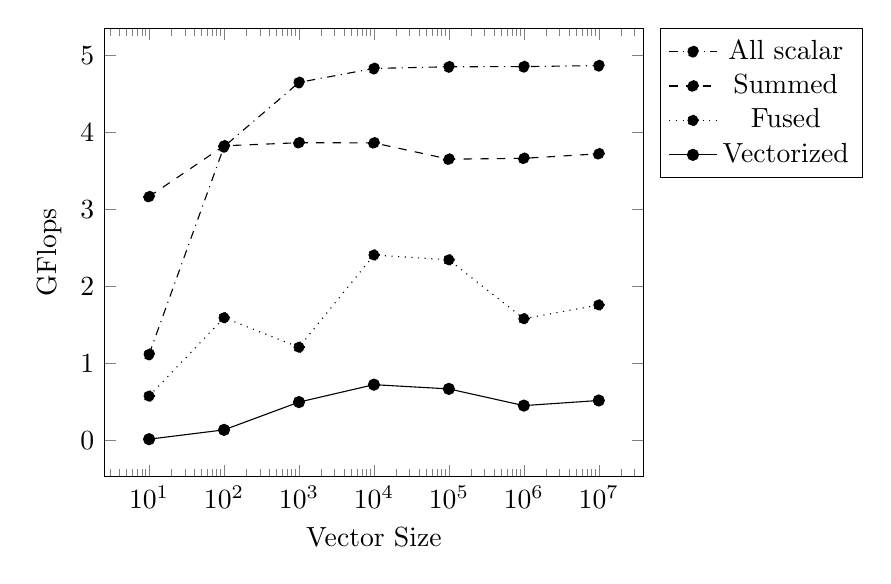
\begin{tikzpicture}
\begin{semilogxaxis}[
    %title=Vectorization Performance,
    xlabel={Vector Size},
    ylabel={GFlops},
    legend entries={Vectorized, Fused, Summed, All scalar},
    legend style={
      %at={(0.98,0.84)},
      legend pos = outer north east,
      anchor = north west,
      reverse legend=true
    },
]
\addplot+[color=black,mark=*,mark options={fill=black}] coordinates {
(10, 0.0181)
(100, 0.1390)
(1000, 0.5001)
(10000, 0.7263)
(100000, 0.6714)
(1000000, 0.4543)
(10000000, 0.5208)

};
\addplot+[color=black,mark=*,mark options={fill=black},style=dotted] coordinates {
(10, 0.5778)
(100, 1.5960)
(1000, 1.2126)
(10000, 2.4110)
(100000, 2.3484)
(1000000, 1.5835)
(10000000, 1.7621)

};
\addplot+[color=black,mark=*,mark options={fill=black},style=dashed] coordinates {
(10, 3.1693)
(100, 3.8297)
(1000, 3.8697)
(10000, 3.8677)
(100000, 3.6557)
(1000000, 3.6670)
(10000000, 3.7258)

};
\addplot+[color=black,mark=*,mark options={fill=black},style=dashdotted] coordinates {
(10, 1.1202)
(100, 3.8186)
(1000, 4.6531)
(10000, 4.8348)
(100000, 4.8566)
(1000000, 4.8585)
(10000000, 4.8718)

};
\end{semilogxaxis}
\end{tikzpicture}
\caption{
\small{
  Performance of evaluating $x^2+x-1$ over a double precision vector of length $n$.
  Operation repeated $10^7/n$ times. (Core i7-3517U 1.9GHz, 4MB cache, 8GB RAM)
}
}
\label{fig:vecperf}
\end{figure}

However, this level of performance is not impressive compared to the
dashed line, which describes the operation rate for computing the
same results but summing them instead of storing them.
Finally, the dash-dotted line uses no memory at all, instead computing
input data points from a linear range.
Of course a real use case might require data to be read from memory or stored,
so this comparison is unfair (though not entirely, since many numerical
environments have represented even simple objects like linear ranges using
dense vectors \cite{matlabman:linspace}).
Still the point should be clear: vectors are not necessarily a good abstraction
for high performance.
The observation that memory is a bottleneck is nothing new, but for our purposes
the important point is that languages that only support vectorized syntax
cannot express the code rearrangements and alternate algorithms that can be
necessary to get the best performance.

The performance model resulting from vectorized syntax can be difficult to
understand, since it is difficult for users to predict which optimizations
will be applied.
A good example was discussed on the \texttt{julia-users} mailing list \cite{jasonmerrill}.
Jason Merrill discovered a Mathematica \cite{mathematica} list discussion
of the fastest way to count how many values fall within a given range.
Of many proposed implementations, the fastest turned out to be

\vspace{-3ex}

\[ \texttt{Total@Unitize@Clip[data,{min,max},{0,0}]} \]

\noindent
Arguably, it is difficult to know that this will run faster than, for
example,

\vspace{-3ex}

\[ \texttt{Count[data,~x\_/;~min<=x<=max]} \]

%% \begin{singlespace}
%% \begin{lstlisting}[language=julia]
%% function count_range(data, min, max)
%%     count = 0
%%     for elt in data
%%         if min < elt < max count += 1 end
%%     end
%%     count
%% end
%% \end{lstlisting}
%% \end{singlespace}

\subsection{Data representation}

Two major approaches:
static language: complex and rigid but efficient memory layout
dyn language: simple but flexible (all pointers)

It's reasonable to guess that these would trade off about equally;
if you want run-time flexibility then it's not worth using complex
specialized data representations.
But this turns out not to be true! It's worth using efficient
memory layouts even if the layout is not known in advance, and you
need an extra dispatch to handle accessing an array (storage strategies).

% ``storage strategies'' is simultaneously a great idea, and also a crack
% in the armor of typical dynamic languages big enough to tear them apart.


\subsection{What needs to be built in?}

On``built-in", why built-in is bad.

Built-in-ness often conflates two aspects:

\begin{enumerate}
\item A feature being readily available and agreed-on by all language users
\item A feature tightly coupled to the rest of the system
\end{enumerate}

(2) implies (1), but not the other way around. (2) is the only technically
interesting item, since the other can be addressed e.g.\  just by including
a library in the standard software distribution. Many technical computing
languages have done a large amount of (2) while justifying it with point (1).


While a large part of our motivation is to move more decisions and functionality
into libraries, it is equally important to identify what {\it must} be part of a
language for the system to be successful. We believe that large amounts of
functionality can be provided by add-ons, but that certain key features
cannot be. Past failures to properly classify features this way have
caused a lot of undue pain.

First, performance cannot be an add-on. If some users have a fast version of
a language and others have a slow version (with the difference being an
order of magnitude or more), library writers cannot be sure whether users
will find their code fast enough to be useful. How are we to teach people to
program in the language?

Psychologically, it may be difficult to accept a ``non standard'' extension
that changes a language so fundamentally. There is a nagging, though perhaps
totally unfounded, perception that something subtle may break. If indeed a
bug arises due to the use of such an extension, a user is likely to conclude
that the extension is dangerous or broken and stop using it. If, on the other
hand, a bug arises due to a language's standard optimizing compiler, the user
will simply file a bug report, then find a way to work around the problem.

Adding a JIT compiler to a language also requires acceptance of detriments
like compilation pauses and pages with RWX permissions. In some cases this
may lead to use of the extension being disallowed, perhaps for security
reasons.

Type systems similarly fail when provided as optional extensions. Library
writers face the same kinds of problems as with performance add-ons. Should I
use type annotations in my library?

Dynamic dispatch mechanisms also make especially poor add-ons. Of course,
every program makes decisions at run time, and so implements its own
``dispatch'' to some extent. But these behaviors are inextensible; if
language users do not agree on a reusable dispatch framework their code
will not be composable.


\section{Code generation}

\begin{itemize}
\item tensor contraction engine
\item Firedrake, pyop2 (vs. c++ libmesh)
\item JuMP vs. python puLP and pyomo
  (want to be able to pass functions, not C++ code as strings)
\item FFTW
\item pochoir
%\item erfinv and horner
\end{itemize}

\subsection{A compiler for every problem}

\cite{hopepython}


\section{Social phenomena}

Programming languages are observed to have strong network effects, and the
difficulty of getting new languages adopted is well known.
However based on \cite{meyerovich2012socio} we believe this doesn't have to
be the case.
The formula of improving or redesigning general-purposes languages to be more
appealing to domain experts might solve the problem.
That way the new system has immediate appeal for at least some users, without
the worry that a different tool will be needed as soon as requirements change
slightly.

Barriers to contributing.

%Debates about what abstractions mean -- AbstractMatrix
%we thought we knew what it meant, but what about something like
%SymTridiagonal? It can implement most of what a dense matrix
%has, but it can't obey every invariant.

%PackedQR

decisions about what to reflect at the type level should be less consequential
somebody might write a c++ library seeking max performance and so
might make array rank a static value.
(we will discuss this further in section~\ref{sec:ndindexing})
somebody else who wants dynamic flexibility might have to write an entirely
separate package.

\chapter{Available technology}

\section{The language design space}

It is helpful to begin with a rather coarse classification of programming
languages, according to how expressive their type systems are, and whether
their type systems are dynamic or static:

\vspace{3ex}

\begin{table}
\begin{tabular}{|c||c|c|}
\hline 
 & More types & Fewer types\tabularnewline
\hline 
\hline 
Dynamic & Dylan, Julia & Scheme, Python, MATLAB\tabularnewline
\hline 
Static & ML, Haskell, Scala & Fortran, Pascal, C\tabularnewline
\hline 
\end{tabular}
\caption[A coarse classification of languages]{}
\label{languageclass}
\end{table}

\vspace{3ex}

The lower right corner tends to contain older languages. The upper right corner
contains many popular ``dynamic'' languages. The lower left corner contains
many modern languages resulting from research on static type systems.
We are most interested in the upper left corner, which is notable for being
rather sparsely populated. It has been generally believed that dynamic
languages do not ``need'' types, or that there is no point in talking about
types if they are not going to be checked at compile time. These views have
some merit, but as a result the top-left corner of this design space has
been under-explored.

\subsection{Classes vs.\ functions}

Technical computing is function oriented.

in C++ to ``extend'' an existing type you have to use another mechanism,
overloading.
however then you also need to accept different semantics, static resolution.


\subsection{Separate compilation vs.\ performance}

Writing the signature of a generic method that needs to be separately compiled,
as in Java, can be a difficult exercise.
The programmer must use the type system to write down sufficient conditions on all
arguments.
The following example from a generic Java graph
library~\cite{Garcia:2003:CSL:949305.949317} demonstrates the level of verbosity
that can be required:

\begin{singlespace}
\begin{lstlisting}[language=java,style=ttcode]
public class breadth_first_search {
  public static<Vertex, Edge extends GraphEdge<Vertex>,
                VertexIterator extends Iterator<Vertex>,
                OutEdgeIterator extends Iterator<Edge>,
                Visitor extends BFSVisitor,
                ColorMap extends ReadWriteMap<Vertex, Integer>>
  void go(VertexListAndIncidenceGraph<Vertex,Edge,
            VertexIterator,VerticesSizeType,OutEdgeIterator,
            DegreeSizeType> g,
          Vertex s, ColorMap c, Visitor vis);
}
\end{lstlisting}
\end{singlespace}

(other problems: primitive types int and double cannot be used,
static parameters can only be inferred directly from arguments,
not from constraints of other parameters. our subtyping system
does not have this problem)

If, however, we are going to specialize the method, the compiler can analyze it
using actual types from call sites, and see for itself whether the method works
in each case (this is how C++ templates are type-checked; they are analyzed
again for each instantiation).

It is quite interesting that performance and ease-of-use pull this design
decision in the same direction.

\subsection{Parametric vs.\ ad-hoc polymorphism}

The term \emph{polymorphism} refers generally to reuse of code or data
structures in different contexts.
A further distinction is often made between \emph{parametric} polymorphism
and \emph{ad-hoc} polymorphism.
Parametric polymorphism refers to reusing the \emph{same} code for
different purposes, while ad-hoc polymorphism refers to selecting
\emph{different} code for different circumstances.

Both forms occur frequently in technical computing.
For example, a programmer intuitively expects that \texttt{A[i]} selects
an element of an array regardless of what kind of array \texttt{A} is.
\texttt{A} might contain integers or strings, it might be a local
array or a distributed array, and so on.
This is parametric polymorphism.
However the ``parametric'' property only applies to the code \texttt{A[i]}
itself.
When we dig into how array indexing actually works, we will probably
need to resort to ad-hoc polymorphism.
For example, when \texttt{A} is a local array the code accesses local
memory, and when \texttt{A} is distributed it might be necessary to
send a network message instead.
At a lower level, the machine code for \texttt{A[i]} needs to be
different depending on the array's element type.

The idea of specialization unites parametric and ad-hoc polymorphism.
Beginning with a parametrically-polymorphic function, one can imagine
a compiler specializing it for various cases, i.e.\ certain concrete argument
values. These specializations could be stored in a lookup table, for use
either at compile time or at run time.

Next we can imagine that the compiler might not optimally specialize
certain definitions, and that the programmer would like to provide
hints or hand-written implementations to speed up special cases.
For example, imagine a function that traverses a generic array. A compiler-generated
specialization might inline a specific array types's indexing operations, but a human
might further realize that the loop order should be switched for certain
arrays types based on their storage order.

However, if we are going to let a human specialize a function for performance,
we might as well allow them to specialize it for some other reason, including
entirely different behavior. But at this point separate ad-hoc polymorphism
is no longer necessary; we are using a single overloading feature for
everything.


Parametric polymorphism describes code that works for any object precisely
because it does not do anything meaningful to the object, for example the
identity function. In contrast, programming with tagged data (e.g.
symbolic expression systems, XML) permits code to work for any object
because every object has the same structure, allowing meaningful
operations.

In theory, a parametrically-polymorphic function works on all data
types.
In practice, this can be achieved by forcing a uniform representation of
data such as pointers, which can be handled by the same code regardless of
what kind of data is pointed to.
However this kind of representation is not the most efficient, and
for good performance specialized code for different types must be
generated.

\subsection{Static checking vs.\ flexibility}

\subsection{Modularity vs.\ large vocabularies}

In the context of software engineering, modularity is a primary concern.
To build large systems, separate components must be isolated to some
degree.
Reasons for this include simple concerns like avoiding name conflicts,
and a desire to separate interface from implementation to allow
a component to change without affecting the rest of the system.

Modularity is sometimes taken to an extreme, and one will see
fully qualified names like \texttt{org.jboss.annotation.ejb.cache.simple.CacheConfig}
(selected from the JBOSS Java APIs).

Technical computing languages have often avoided and discouraged such
designs. For example MATLAB for most of its history supported only a single
namespace, which comes pre-populated with thousands of functions.


\subsection{Eliminating vs.\ embracing tagged data}

\subsection{Data hiding vs.\ explicit memory layout}

Examples of CSC and CSR sparse representation.
In one sense this is a perfect example of an interface with multiple implementations,
and therefore a good use case for object-oriented programming.
However in the technical computing world, \emph{hiding} this difference in
representation is not usually considered desirable.
Clearly a sparse matrix class cannot contain all functions of matrices that users
might want to compute.
Yet when new functions are added, the programmer needs and wants to exploit
representation details (CSC or CSR) for performance.
The performance differences involved here are quite significant (TODO cite).

The loss of encapsulation due to multi-methods weighed in \cite{binarymethods}
is less of a problem for technical computing, and in some cases even
advantageous.

\subsection{Dynamic dispatch is key}

It would be unpleasant if every piece of every program we wrote were forced
to do only one specific task. Every time we wanted to do something slightly
different, we'd have to write a different program. But if a language
allows the same program element to do different things at different times,
we can write whole classes of programs at once. This kind of capability is
one of the main reasons \emph{object-oriented} programming is popular: it
provides a way to automatically select different behaviors according to
some structured criteria.

In class-based OO there is essentially \emph{no way} to create an operation
that dispatches on existing types (the expression problem \cite{wadler1998expression}).
This clearly
does not match technical computing, where most programs deal with the same
few types (e.g. number, array), and might sensibly want to write new operations
that dispatch on them.

%Somewhat unfortunately, the term \emph{object-oriented} has many
%connotations, and the \emph{object-oriented} methodology tries to address
%multiple software engineering problems --- for example modularity,
%encapsulation, implementation hiding, and code reuse. These issues are
%important, but it may be because of them that over time too little
%emphasis has been placed on expressive power.

We use the non-standard term ``criteria'' deliberately, in order
to clarify our point of view, which is independent of any particular
object system.

The sophistication of the available ``selection criteria'' account for a
large part of the perceived ``power'' or leverage provided by a language.
In fact it is possible to illustrate a hierarchy of such mechanisms.
As an example, consider a simple simulation, and how it can be written
under a series of increasingly powerful paradigms. First, written-out
imperative code:

\begin{singlespace}
\begin{verbatim}
while running
    for a in animals
        b = nearby_animal(a)
        if a isa Rabbit
            if b isa Wolf then run(a)
            if b isa Rabbit then mate(a,b)
        else if a isa Wolf
            if b isa Rabbit then eat(a,b)
            if b isa Wolf then follow(a,b)
        end
    end
end
\end{verbatim}
\end{singlespace}

We can see how this would get tedious as we add more kinds of animals
and more behaviors. Another problem is that the animal behavior is
implemented directly inside the control loop, so it is hard to see
what parts are simulation control logic and what parts are animal
behavior. Adding a simple object system leads to a nicer implementation
\footnote{A perennial problem with simple examples is that better
implementations often make the code longer.}:

\begin{singlespace}
\begin{verbatim}
class Rabbit
    method encounter(b)
        if b isa Wolf then run()
        if b isa Rabbit then mate(b)
    end
end

class Wolf
    method encounter(b)
        if b isa Rabbit then eat(b)
        if b isa Wolf then follow(b)
    end
end

while running
    for a in animals
        b = nearby_animal(a)
        a.encounter(b)
    end
end
\end{verbatim}
\end{singlespace}

Here all of the simulation's animal behavior has been essentially
compressed into a single program point: \texttt{a.encounter(b)}
leads to all of the behavior by selecting an implementation based
on the first argument, \texttt{a}. This kind of criterion is
essentially indexed lookup; we can imagine that \texttt{a} is
simply an integer index into a table of operations.

The next enhancement to ``selection criteria'' adds a hierarchy
of behaviors, to provide further opportunities to avoid
repetition:

\todo[inline]{has  $<:$  been defined yet?}

\begin{singlespace}
\begin{verbatim}
abstract class Animal
    method nearby()
        # search within some radius
    end
end

class Rabbit <: Animal
    method encounter(b: Animal)
        if b isa Wolf then run()
        if b isa Rabbit then mate(b)
    end
end

class Wolf <: Animal
    method encounter(b: Animal)
        if b isa Rabbit then eat(b)
        if b isa Wolf then follow(b)
    end
end

while running
    for a in animals
        b = a.nearby()
        a.encounter(b)
    end
end
\end{verbatim}
\end{singlespace}

We are still essentially doing table lookup, but the tables have
more structure: every \texttt{Animal} has the \texttt{nearby}
method, and can inherit a general-purpose implementation.

This brings us roughly to the level of most popular object-oriented
languages. But in this example still more can be done. Notice that
in the first step to objects we replaced one level of \texttt{if}
statements with method lookup. However, inside of these methods
a structured set of \texttt{if} statements remains. We can
replace these by adding another level of dispatch.

\begin{singlespace}
\begin{verbatim}
class Rabbit <: Animal
    method encounter(b: Wolf) = run()
    method encounter(b: Rabbit) = mate(b)
end

class Wolf <: Animal
    method encounter(b: Rabbit) = eat(b)
    method encounter(b: Wolf) = follow(b)
end
\end{verbatim}
\end{singlespace}

We now have a \emph{double dispatch} system, where a method call
uses two lookups, first on the first argument and then on the
second argument.

This syntax might be considered a bit nicer, but the design
clearly begs a question: why is $n=2$ special? It isn't, and we
could clearly consider even more method arguments as part of
dispatch. But at that point, why is the first argument special?
Why separate methods in a special way based on the first argument?
It seems arbitrary, and indeed we can remove the special treatment:

\begin{singlespace}
\begin{verbatim}
abstract class Animal
end

class Rabbit <: Animal
end

class Wolf <: Animal
end

nearby(a: Animal) = # search
encounter(a: Rabbit, b: Wolf) = run(a)
encounter(a: Rabbit, b: Rabbit) = mate(a,b)
encounter(a: Wolf, b: Rabbit) = eat(a, b)
encounter(a: Wolf, b: Wolf) = follow(a, b)

while running
    for a in animals
        b = nearby(a)
        encounter(a, b)
    end
end
\end{verbatim}
\end{singlespace}

Here we made two major changes: the methods have been moved ``outside''
of any classes, and all arguments are listed explicitly. This change
has fairly significant implications. Since methods no longer need to be
``inside'' classes, there is no syntactic limit to where definitions
may appear. Now it is easier to add new methods after a class has
been defined. Methods also now naturally operate on combinations of
objects, not single objects.

The shift to thinking about combinations of objects is fairly
revolutionary. Many interesting properties only apply to combinations
of objects, and not individuals. We are also now free to think of
more exotic kinds of combinations.

We can define a method on \emph{any number} of objects:

\begin{verbatim}
encounter(ws: Wolf...) = pack(ws)
\end{verbatim}

\todo[inline]{We can also do diagonal dispatch:}

\begin{verbatim}
encounter{T<:Animal}(a: T, b: T) = mate(a, b)
\end{verbatim}



\section{Dispatch systems}

% CHART of different multiple dispatches. classify them

%Why ``just overloading'' is not enough. You intercept every operation and
%rewrite it, kind of an escape hatch for a language you don't like. If
%somebody else also tries to do this, there won't necessarily be any
%coherence.

A helpful way to classify languages with some kind of generic programming
support is to look at which language constructs are generic. For example,
in C++ the syntax \texttt{object.method(x)} is generic: a programmer can
get it to do different things by supplying different values for
\texttt{object}. The C++ syntax \texttt{f(a,b)} or \texttt{a+b} is
usually not generic, but can be overloaded by supplying definitions for
different argument types. However, this overloading only uses compile time
types (no run time information), and so is essentially a form of renaming ---
it can be implemented by renaming each definition with a unique name, and
replacing overloaded calls with an appropriate name based on compile time
types. This is a much weaker form of generic programming, since different
behaviors cannot be obtained by passing different values at run time.

For this reason, C++ programs are not fully generic: it is difficult to
substitute new behaviors for every part of a program. Some languages
take generic programming much further. For example, in MATLAB, \emph{every}
function is effectively generic, and can be overloaded by new classes.
This enables a programmer to ``intercept'' every function call (and therefore,
essentially everything a program does)


\subsection{Example: lattices}

This example will illustrate possible benefits of multiple dispatch and
dynamic typing for mathematical computing.
The benefits are not absolute, but notational and semantic:
they involve code size and clarity, and the extent to which the entities
provided by the language match a mental model of the domain.

A \emph{lattice} is an algebraic structure where some pairs of elements
satisfy a reflexive, antisymmetric, and transitive relation $\leq$.
For purposes of this example, we will consider lattices that have
a greatest, or \emph{top}, element ($\top$), and a least, or \emph{bottom}
element ($\bot$). When working with lattices one often wants to compute
a least upper bound, or \emph{join} ($\sqcup$), or a greatest lower bound,
or \emph{meet} ($\sqcap$).

Several interesting concerns arise when modeling lattices in a programming
language. First, the structure is very general, and so admits implementations
for many different kinds of elements. We want to write code using
the operators $\leq$, $\sqcup$, and $\sqcap$, and have it apply to any kind
of lattice. Therefore some kind of overloading or object-oriented programming
is desirable. Second, some properties apply to all lattices, and we would
like to avoid implementing them repeatedly.

Using ``duck typing'', the problem of modeling an abstraction like lattices
disappears almost entirely. One may simply define methods for
$\leq$, $\sqcup$, and $\sqcap$ at any time, for any type, and that type will
function as a lattice. That is certainly convenient, but it also fails to
provide any reusable functionality for those defining lattices.



\begin{figure}[!t]
\todo[inline]{what does $===$ mean here?}  
  \begin{center}
\begin{singlespace}
\begin{lstlisting}[language=julia]
abstract LatticeElement

<=(x::LatticeElement, y::LatticeElement) = x===y
==(x::LatticeElement, y::LatticeElement) = x<=y && y<=x
< (x::LatticeElement, y::LatticeElement) = x<=y && !(y<=x)

immutable TopElement <: LatticeElement; end
immutable BotElement <: LatticeElement; end

const ~$\top$~ = TopElement()
const ~$\bot$~ = BotElement()

<=(::BotElement, ::TopElement) = true
<=(::BotElement, ::LatticeElement) = true
<=(::LatticeElement, ::TopElement) = true



~$\sqcup$~(x::LatticeElement, y::LatticeElement) =  # join
    (x <= y ? y : y <= x ? x : ~$\top$~)

~$\sqcap$~(x::LatticeElement, y::LatticeElement) =  # meet
    (x <= y ? x : y <= x ? y : ~$\bot$~)
\end{lstlisting}
\end{singlespace}
  \end{center}
  \label{julialattices}
  \caption{A small Julia library for lattices}
\end{figure}





Figure~\ref{julialattices} shows a small Julia library for lattices.
It defines an abstract class \texttt{LatticeElement} that may be subclassed
by objects that will be used primarily as elements of some lattice.
The library also provides standard
\texttt{LatticeElement} provides some useful default method definitions.\todo{sentence grammar?}
\todo[inline]{Join of two incomparables in general lattices does not have to be top}



\subsection{Symbolic programming}

There has always been an essential divide between ``numeric'' and ``symbolic''
languages in the world of technical computing. To many people the
distinction is fundamental, and we should happily live with both
kinds of languages. But if one insists on an answer as to which approach
is the right one, then the answer is: \todo{Love it!}  symbolic.

Systems based on symbolic rewrite rules arguably occupy a further tier of
dispatch sophistication. In these systems, you can dispatch on essentially
anything, including arbitrary values and structures. These systems are
typically powerful enough to concisely define the kinds of behaviors we
are interested in.

However, symbolic programming lacks data abstraction: the concrete
representations of values are exposed to the dispatch system
(e.g. there is no difference between being a list and being something
represented as a list).
\todo{Wish you would say more!}

\subsection{Predicate dispatch}

%Patterns are very powerful, but the tradeoff is that there is not
%necessarily a useful relationship between what your program does and
%what a static analysis (based on a finite-height partial order over
%patterns) can discover. Maybe julia could be considered a sweet spot
%somewhere in between.

Predicate dispatch is a powerful object-oriented mechanism that allows
methods to be selected based on arbitrary predicates \cite{ErnstKC98}.
It is, in some
sense, the most powerful \emph{possible} dispatch system, since any
computation may be done as part of method selection. Since a predicate
denotes a set (the set of values for which it is true), it also denotes
a set-theoretic type. Some type systems of this kind, notably that of
Common Lisp \cite{steele1990common:types}, have actually included predicates as types.
However, such a type system is obviously undecidable, since it
requires computing the predicates themselves or, even worse, computing
predicate implication.\footnote{
Many type systems involving bounded quantification, such as system $F_{<:}$,
are already undecidable \cite{Pierce1994131}.
However, they seem to terminate for most practical programs, and also admit
minor variations that yield decidable systems \cite{Castagna:1994:DBQ:174675.177844}.
It is fair to say they are ``just barely'' undecidable, while predicates
are ``very'' undecidable.
}

For a language that is willing to do run time type checks anyway, the
undecidability of predicate dispatch is not a problem.
Interestingly, it can also pose no problem for \emph{static} type systems
that wish to prove that every call site has an applicable method.
Even without evaluating predicates, one can prove that the available methods
are exhaustive (e.g. methods for both $p$ and $\neg p$ exist).
In contrast, and most relevant to this thesis, predicate types \emph{are} a
problem for code \emph{specialization}. Static method lookup would require
evaluating the predicates, and optimal code generation would require
understanding something about what the predicates mean. One approach would
be to include a list of satisfied predicates in a type. However, to the
extent such a system is decidable, it is essentially equivalent to multiple
inheritance. Another approach would be to separate predicates into a
second ``level'' of the type system. The compiler would combine methods
with the same ``first level'' type, and then generate branches to evaluate
the predicates. Such a system would be very useful, and could be
% TODO cite, as this has probably been done
combined with a language like Julia or, indeed, most object-oriented
languages. However this comes at the expense of conceding that predicates
are not ``real'' types.

In considering the problems of predicate dispatch for code specialization,
we seem to be up against a fundamental obstacle: some sets of values are
simply more robust under evaluation than others. Programs that map integers
to integers abound, but programs that map, say, even integers to even
integers are rare to the point of irrelevance.


\section{Domain theory}

In the late 1960s Dana Scott and Christopher Strachey asked how to assign
meanings to programs, which otherwise just appear to be lists of symbols
\cite{scott1971toward}.
For example, given a program computing the factorial function, we
want a process by which we can assign the meaning ``factorial'' to it.
This led to the invention of domain theory, which can be interpreted
as modeling the behavior of a program without running it.
A ``domain'' in this theory is a
partial order of sets of values that a program might manipulate. 
Domain theory models computation as follows: a program starts with no
information, the lowest point in the partial order (``bottom'').
Computation steps accumulate information, gradually moving higher through
the order. The advantage of this model, in essence, is that it provides a
way to think about the meaning of a program without running the program.
Even the ``result'' of a non-terminating program has a representation ---
the bottom element. Other elements of the partial order might refer to
intermediate results.

The idea of ``running a program without running it'' is of great interest
in compiler implementation. A compiler would like to discover as much
information as possible about a program without running it, since
running it might take a long time, or produce side effects that the
programmer does not want yet, or, of course, not terminate.
The general recipe for doing this is to design a partial order (lattice)
that captures program properties of interest, and then describe all
primitive operations in the language based on how they transform
elements of this lattice.
Then an input program can be executed, in an approximate sense, until
it converges to a fixed point.
For example, given a program that outputs an integer, we might decide
that we only care whether this integer is even or odd. Then our posets
are the even and odd integers, and we will classify operations in the
program according to whether they are evenness-preserving,
evenness-inverting, always even, always odd, of uncertain evenness,
etc. % TODO figure
Most modern compilers use a technique like this
(sometimes called abstract interpretation \cite{abstractinterp})
to semi-decide
interesting properties like whether a variable is a constant, whether
a variable might be used before it is initialized, whether a variable's
value is never used, and so on.
%Domain theory gave rise to the study of denotational semantics and the
%design of type systems. However, the original theory is quite general
%and invites us to invent any domains we wish for any sort of language.
%Abstract interpretation \cite{abstractinterp} is an especially
%elegant and general implementation of this idea.
%It should be clear that this sort of analysis, while clearly related
%to type systems, is fairly different from what most programmers
%think of as type \emph{checking}.

Given the general undecidability of questions about programs, analyses
like these are \emph{conservative} in nature.
For example, if our goal is to warn programmers about use of uninitialized
variables, we want to be ``better safe than sorry'' and print a warning
if such a use \emph{might} occur.
Such a use corresponds to any lattice element greater than or equal to
the element representing ``uninitialized''.
Such conservative analyses are the essence of compiler transformations
for performance (optimizations): we only want to perform an optimization
if the program property it relies on holds for sure, and not if there is
any uncertainty.

The generality of this approach makes it a kind of ``ur type system'':
we can discover a large variety of program properties as long as we are
willing to accept some uncertainty.
Of course, many programmers and language designers prefer to maximize
safety, leading to different approaches that trade away some precision
(e.g. syntactic type systems such as those in the ML language
family \cite{hindley1969principal}, \cite{MLtypeinf}).
But if static guarantees are not the priority, or if a language considers
itself unconcerned with ``types'', then we can take the domain-theoretic
model as our type system.
In some sense, it is our type system whether we like it or not
(as implied by \cite{scott1976data})!

\subsection{Monotonicity}

When this kind of type system is used, it usually becomes part of the
meta-theory of the language: values are ``lifted'' into an abstract
domain, and abstract values are manipulated only by a compiler
or other program analysis.
One good reason for this is that the abstract values (which we will
now interchangeably call ``types'') must meet certain requirements in
order to be useful.
For an abstract interpretation to terminate, its lattice must be of
finite height, and all functions of lattice elements must be
monotonic (given lattice elements $a$ and $b$, we must have
$a\subseteq b$ implies $f(a)\subseteq f(b)$ for all $f$).


Functions of types are not monotonic. \texttt{isa(2,3)} is \texttt{false},
but \texttt{isa(2,Int)} is \texttt{true}.
This provides one way to separate ``real types'' from set-valued terms:
if there is a way to interpret execution over types such that all functions
are monotonic in the (alleged) type lattice, then we are really dealing
with types.
One way to do this is to specify a genuinely multi-valued term language
like $\lambda_\aleph$ \cite{Glew:2013:MLD:2502409.2502412}.
In this approach a term like \texttt{isa(2,Int)} is interpreted as a
union of all results obtained by substituting all possible single values
for each sub-term. One cannot help but be impressed by such a language,
though it seems prohibitively difficult to actually implement.
%$\lambda_\aleph$ was introduced a couple years after we began work on Julia
We opt instead for a simpler approach where \texttt{Int} is
interpreted as \texttt{Type\{Int\}} (in a near-borrowing of notation from
\cite{Glew:2013:MLD:2502409.2502412} and \cite{cardelli1986polymorphic}),
and multi-valued terms exist only statically within a separate
maximum-fixed-point evaluator.

\section{Subtyping}

Something about semantic subtyping and type systems for processing XML.
XML at first seems unrelated to numerical computing, and indeed it
was quite a while before we discovered these papers and noticed the
overlap. However if one substitutes ``symbolic expression'' for
``XML document'', the similarity becomes clearer.

% maybe subarray as an example of a fancy type here


%% \subsection{Objections to dynamic typing}

% there are run time things, and just flow-sensitive things

% coming up with examples where something needs to be done at
% run time seems to be difficult. as soon as a concrete example
% is raised, one immediately imagines doing it statically.


%% it may be that the ``power'' of a language is equal to the complexity
%% of the criteria used by the language's run time dispatch mechanisms.

%% pre-OO: pointer indirection
%% OO: single dispatch, class hierarchies

%% Haskell: without typeclasses, a beautiful language, but one that nobody
%% would use.

%% I claim that compile time abstractions do not count. The problem is that
%% at some point you have to *actually run the program*. Specifying the
%% behavior of a program is hard; this is where we need help from the
%% language.

%% Scripting languages are often defended using the observation that most
%% code is not performance-critical. However, this fact does not mean that
%% it's ok for a language design to ignore performance, nor does it mean
%% that performance should be the default priority of every line of code.
%% Rather it means that the default should be convenience and safety, with
%% a path to performance easily in reach for when it's needed.

\chapter{Case studies}

\section{Explication through elimination}

This section will illustrate how we implement key features of technical computing
systems using our methodology.

\subsection{Conversion and comparison}

Type conversion provides a classic example of a binary method. Multiple
dispatch allows us to avoid deciding whether the converted-to type or the
converted-from type is responsible for defining the operation.
Defining a specific conversion is straightforward, and might look like this
in Julia syntax:

\begin{verbatim}
convert(::Type{Float64}, x::Int32) = ...
\end{verbatim}

\noindent
A call to this method would look like \texttt{convert(Float64, 1)}.

Using conversion in generic code requires more sophisticated definitions.
For example we might need to convert one value to the type of another,
by writing \texttt{convert(typeof(y), x)}. What set of definitions must
exist to make that call work in all reasonable cases? Clearly we cannot
explicitly write all $O(n^2)$ possibilities. We need abstract definitions
that cover many points in the dispatch matrix. One such family of points
is particularly important: those that describe converting a value to a
type it is already an instance of. In our system this can be handled by
a single definition that performs ``triangular'' dispatch:

\begin{verbatim}
convert{T}(::Type{T}, x::T) = x
\end{verbatim}

\noindent
``Triangular'' refers to the rough shape of the dispatch matrix covered
by such a definition: for all types \texttt{T} in the first argument slot,
match any type less than it in the second argument slot.


- The abstractions of equality and comparison. Different equivalence classes between

is/===, isequal and ==

- Numeric vs lexicographic ordering?

cmp, lexcmp, vs isless, <

\subsection{Numeric types and embeddings}

We might prefer ``number'' to be a single,
concrete concept, but the history of mathematics has seen the concept
extended many times, from integers to rationals to reals, and then to complex,
quaternion, and more. These constructions tend to follow a pattern: a new set
of numbers is constructed around a subset isomorphic to an existing set of
numbers. For example, the reals are isomorphic to the complex numbers with
zero imaginary part.

Human beings happen to be good at equating and moving between isomorphic sets,
so it is easy to imagine that the reals and complexes with zero imaginary
part are one and the same. But a computer forces us to be specific, and admit
that a real number is not complex, and a complex number is not real. And yet
the close relationship between them is too compelling not to model in a
computer somehow. Here we have a numerical analog to the famous ``circle and
ellipse'' problem in object-oriented programming: the set of circles is
isomorphic to the set of ellipses with equal axes, yet neither ``is a''
relationship in a class hierarchy seems fully correct. An ellipse is not
a circle, and in general a circle cannot serve as an ellipse (for example,
the set of circles is not closed under the same operations that the set of
ellipses is, so a program written for ellipses might not work on circles).
This problem implies that a single built-in type hierarchy is not
sufficient: we want to model custom *kinds* of relationships between
types (e.g. ``can be embedded in'' in addition to ``is a'').

Two further problems should also be kept in mind. First, the natural isomorphisms
between sets of numbers might not be isomorphisms on a real computer. For example,
due to the behavior of floating-point arithmetic, an operation on complex numbers
with zero imaginary part might not give an answer equal to the same operation on
real numbers. Second, the contexts that demand use of one type of number or
another are often not easily described by type systems. The classic example is
square root (\texttt{sqrt}), whose result is complex for negative arguments.
Including a number's sign in its type is a possibility, but this quickly gets
out of hand --- should a type system attempt to prove a matrix symmetric before
we compute its eigenvalues? While we cannot offer a once-and-for-all solution
to these problems, we will show how the flexibility of our proposed mechanism
is useful for addressing them.

% ex: generic sum function accumulating result in at least
% double precision. just using +::T->T->T doesn't work.

\subsubsection{Implementing type embeddings}

Most functions are naturally implemented in the value domain, but some are
actually easier to implement in the type domain. One reason is that there
is a bottom element, which most data types lack.

\subsubsection{Diversity of number and number-like types in practice}

Originally, our reasons for implementing all numeric types at the library
level were not entirely practical. We had a principled opposition to
including such definitions in a compiler, and guessed that being able to
define numeric types would help ensure the language was ``powerful enough''.
However, defining numeric and number-like types and their interactions turns
out to be surprisingly useful. Once such types become easy to obtain,
people find more and more uses for them.

Ordinal types: Pointer, Char

Integer types: Int8, Int16, Int32, Int64, Int128, UInt8, UInt16, UInt32, UInt64, UInt128, BigInt

Floating point types: Float16, Float32, Float64, BigFloat
(Float128, double-double)

Fixed point: Fixed32{b}, Ufixed8, Ufixed16

Extensions: Complex, Quaternion, Interval, DualNumber

Number-like: Date, TimePeriod, DatePeriod, Color, (Units), DNA nucleotide type (bioseq.jl)
dates: different cardinal and ordinal behavior

musical notes

\subsubsection{Applications}

\emph{Ranges} illustrate an interesting application of type promotion.
A range data type, notated \texttt{a:s:b}, represents a sequence of values
starting at \texttt{a} and ending at \texttt{b}, with a distance of \texttt{s}
between elements (internally, this notation is translated to
\texttt{colon(a, s, b)}). Ranges seem simple enough, but a reliable,
efficient, and generic implementation is difficult to achieve.
We propose the following requirements:

\begin{itemize}
\item The start and stop values can be passed as different types, but internally
  should be of the same type.
\item Ranges should work with ordinal types, not just numbers (examples include
  characters, pointers, and calendar dates).
\item If any of the arguments is a floating-point number, a special
  \texttt{FloatRange} type designed to cope well with roundoff is returned.
\end{itemize}

In the case of ordinal types, the step value is naturally of a different type
than the elements of the range. For example, one may add 1 to a character to
get the ``next'' encoded character, but it does not make sense to add two
characters.

It turns out that the desired behavior can be achieved with six definitions:

First, given three floats of the same type we can construct a \texttt{FloatRange}
right away:

\begin{verbatim}
colon{T<:FloatingPoint}(start::T, step::T, stop::T) = FloatRange{T}(start, step, stop)
\end{verbatim}

Next, if \texttt{a} and \texttt{b} are of the same type and there are no floats,
we can construct a general range:

\begin{verbatim}
colon{T}(start::T, step, stop::T) = StepRange(start, step, stop)
\end{verbatim}

Now there is a problem to fix: if the first and last arguments are of some
non-floating-point numeric type, but the step is floating point, we want to
promote all arguments to a common floating point type. We must also do this
if the first and last arguments are floats, but the step is some other kind
of number:

\begin{verbatim}
colon{T<:Real}(a::T, s::FloatingPoint, b::T) = colon(promote(a,s,b)...)

colon{T<:FloatingPoint}(a::T, s::Real, b::T) = colon(promote(a,s,b)...)
\end{verbatim}

These two definitions are correct, but ambiguous: if the step is a float
of a different type than \texttt{a} and \texttt{b} both definitions are
equally applicable. We can add the following disambiguating definition:

\begin{verbatim}
colon{T<:FloatingPoint}(a::T, s::FloatingPoint, b::T) = colon(promote(a,s,b)...)
\end{verbatim}

All of these five definitions require \texttt{a} and \texttt{b} to be of the
same type. If they are not, we must promote just those two arguments, and leave
the step alone in case we are dealing with ordinal types:

\begin{verbatim}
colon{A,B}(a::A, s, b::B) = colon(convert(promote_type(A,B),a), s, convert(promote_type(A,B),b))
\end{verbatim}

This example shows that it is not always sufficient to have a built-in set of
``promoting operators''. Library functions like this \texttt{colon} need more
control.


\subsubsection{Current approaches}

Numbers tend to be among the most
complex features of a language. Numeric types usually need to be a special
case: in a typical language with built-in numeric types, describing their
behavior is beyond the expressive power of the language itself. For example,
in C arithmetic operators like \texttt{+} accept multiple types of arguments
(ints and floats), but no user-defined C function can do this (this situation
is of course improved in C++). In Python, a special arrangement is made for
\texttt{+} to call either an \texttt{\_\_add\_\_} or \texttt{\_\_radd\_\_} method,
effectively providing double-dispatch for arithmetic in a language that is
idiomatically single-dispatch.



\subsection{Multidimensional array indexing}

One-dimensional arrays are a simple and essential data structure found in
most programming languages. The multi-dimensional arrays required in
scientific computing, however, are a different beast entirely. Allowing
any number of dimensions entails a significant increase in complexity. Why?
The essential reason is that core properties of the data structure no
longer fit in a constant amount of space. The space needed to store the
sizes of the dimensions (the array shape) is proportional to the number
of dimensions. This does not seem so bad, but becomes a large problem
due to three additional facts.

% TODO: break up using enumerate
First, code that operates on the dimension
sizes needs to be highly efficient. Typically the overhead of a loop is
unacceptable, and such code needs to be fully unrolled. Second, in some
code the number of dimensions is a \emph{dynamic} property --- it is
only known at run time. Third, programs may wish to treat arrays with
different numbers of dimensions very differently. A vector (1d) might
have rather different behaviors than a matrix (2d) (for example, to
compute a norm). This kind of
behavior makes the number of dimensions a crucial part of program
semantics, preventing it from remaining a compiler implementation detail.

% TODO: break up using enumerate
These facts pull in different directions. The first fact asks for static
analysis. The second fact asks for run-time flexibility. The third fact asks
for dimensionality to be part of the type system, but partly determined
at run time (for example, via virtual method dispatch). Current approaches
choose a compromise. In some systems, the number of dimensions has a strict
limit (e.g. 3 or 4), so that separate classes for each case may be written
out in full. Other systems choose flexibility, and just accept that most
or all operations will be dynamically dispatched. Other systems might
provide flexibility only at compile time, for example a template library
where the number of dimensions must be statically known.

%% TODO: insert example of limited power of C++ array libraries

%% TODO: examples of systems limited to n==3

Whatever decision is made, rules must be defined for how various operators
act on dimensions. For now we will focus on indexing, since selecting
parts of arrays has particularly rich behavior with respect to
dimensionality. For example, if a single row or column of a matrix is
selected, does the result have one or two dimensions? Array implementations
prefer to invoke general rules to answer such questions. Such a rule might
say ``dimensions indexed with scalars are dropped'', or ``trailing
dimensions of size one are dropped'', or ``the rank of the result
is the sum of the ranks of the indexes'' (as in APL).

%%%
Our goal here is a bit unusual: we are not concerned with which rules
might work best, but merely with how they can be specified, so that
domain experts can experiment.

In fact different domains want different things. E.g. in images, each
dimension might be quite different, e.g. time vs. space vs. color,
so you don't want to drop or rearrange dimensions very often.
%%%

Here are our ground rules:

\begin{enumerate}
\item You can't manually implement the behavior inside the compiler
\item The compiler must be able to reasonably understand the program
\item The code must be reasonably easy to write
\end{enumerate}


How are such rules implemented? For a
language with built-in multidimensional arrays, the compiler will
analyze indexing expressions and determine an answer using hard-coded
logic.
% TODO: grab example from one of these compilers
However, this approach is not satisfying: we would rather
implement the behavior in libraries, so that different kinds of arrays
may be defined, or so that rules of similar complexity may be
defined for other kinds of objects. But these kinds of rules are
unusually difficult to implement in libraries. If a library writes out
its indexing logic using imperative code, the host language compiler
is not likely to be able to analyze it. Using compile-time abstracton
(templates) would provide better performance, but such libraries tend
to be difficult to write (and read), and the full complement of
indexing behavior expected by technical users strains the capabilities
of such systems.

% TODO: insert actual example of numpy

Our dispatch mechanism permits a novel solution. If a multiple dispatch
system supports variadic functions and argument ``splicing'' (the ability
to pass a structure of $n$ values as $n$ separate arguments to a function),
then indexing behavior can be defined as method signatures.

This solution is still a compromise among the factors outlined above,
but it is a new compromise that provides a net-better solution.
% TODO more

Below we define a function \texttt{index\_shape} that computes the
shape of a result array given a series of index arguments. We show
three versions, each implementing a different rule that users in
different domains might want:

% TODO: point out array = (shape, data), so those are the two parts
% we need to handle. In julia the ``data'' part is not a first class
% object; it is not directly exposed to the user, but this is more
% of an implementation detail.

\begin{verbatim}
# drop dimensions indexed with scalars
index_shape() = ()
index_shape(i::Real, I...) = index_shape(I...)
index_shape(i, I...) = tuple(length(i), index_shape(I...)...)
\end{verbatim}

\begin{verbatim}
# drop trailing dimensions indexed with scalars
index_shape(i::Real...) = ()
index_shape(i, I...) = tuple(length(i), index_shape(I...)...)
\end{verbatim}

\begin{verbatim}
# rank summing (APL)
index_shape() = ()
index_shape(i, I...) = tuple(size(i)..., index_shape(I...)...)
\end{verbatim}

Inferring the length of the result of \texttt{index\_shape} is sufficient
to infer the rank of the result array.

These definitions are concise, easy to write, and possible for a
compiler to understand fully using straightforward techniques.

% TODO: point out how this combines the ``object part'' and the
% ``array part'' into a coherent whole.

Here is a sample derivation for the call \texttt{index\_shape(1:m,1,1:n)}
(the argument type tuple is \texttt{(Range1,Int,Range1)}), using the first
definition above (dropping scalar-indexed dimensions):

\begin{verbatim}
index_shape(1:n, 1, 1:m) => tuple(length(::Range1)::Int, index_shape((::Int, ::Range1)...)...)

index_shape((::Int, ::Range1)...) => index_shape(::Int, ::Range1)

index_shape(::Int, ::Range1) => index_shape((::Range1,)...)

index_shape((::Range1,)...) => index_shape(::Range1)

index_shape(::Range1) => tuple(length(::Range1)::Int, index_shape(()...)...)

index_shape(()...) => index_shape()::()

back substitute => tuple(length(::Range1)::Int, index_shape(()...)::()...)::(Int,)

back substitute => tuple(length(::Range1)::Int, ::(Int,)...)

tuple(::Int, ::(Int,)...) => tuple(::Int, ::Int)

::(Int, Int)

\end{verbatim}

The result type is determined using only dataflow type inference, plus a
rule for splicing an immediate container (the type of \texttt{f((a,b)...)} is
the type of \texttt{f(a,b)}). Argument list destructuring takes place inside
the type intersection operator used to combine argument types with method
signatures.

This approach does not depend on any heuristics. Each call to \texttt{index\_shape}
simply requires one recursive invocation of type inference. This process reaches
the base case \texttt{()} for these definitions, since each recursive call
handles a shorter argument list (for less-well-behaved definitions, we might
end up invoking a widening operator instead).


\begin{verbatim}
diverge() = randbool() ? () : tuple(1, diverge()...)
\end{verbatim}

\subsection{Array views}

\subsection{Units}

\subsection{Even more elimination?}

Some features of the language could be even further eliminated. For example data
types could be implemented in terms of lambda abstractions. But certain patterns
are so useful that they might as well be provided in a standard form. It also
probably makes the compiler much more efficient not to need to pass around and
repeatedly analyze full representations of the meanings of such ubiquitous constructs.


\section{Numerical linear algebra}

Multiple dispatch on special matrices

29 LAPACK types via composition of 9 types, issue 8240


\section{Boundary-element method}

There are lots of general packages for FEM problems, but it is much more
difficult to create such a package for BEM problems. The method requires
integrating functions with singularities, many times in the inner loop
of code that builds the problem matrix. Integrating such functions
numerically on each iteration is much too slow. As a result, many
special-purpose implementations have been written by hand for different
problems.

Some recent work (TODO cite Homer) managed a more general solution,
using Mathematica to generate C++ code for different cases. This worked
well, but was difficult to implement and the resulting system is difficult
to use. We see the familiar pattern of using multiple languages and
code-generation techniques, with coordination of the overall process done
either manually or with ad-hoc scripts. To polish the implementation for
use as a practical library, a likely next step would be to add a Python
interface, adding yet another layer of complexity.


Features of julia this demonstrates:

- functions that need to dispatch on more than one argument
- staged methods providing a natural way to integrate code generation
- doing specialization through the object system, leading to a ``flat'' system

The code can be structured as a simple function library.

%%%%%%%%%%%%%%%%%%%%%%%%%%%%%%%%%%%%%%%%%%%%%%%%%%%%%%%%%%%%%%%%%%%%%%%%%%%

% writeup by SGJ

\subsection{Galerkin matrix assembly for singular kernels}

A typical problem in computational science is to form a discrete approximation of some infinite-dimensional linear operator $\mathcal{L}$ with some finite set of basis functions $\{ b_m \}$ via a Galerkin approach [refs], which leads to a matrix $L$ with entries $L_{mn} = \langle b_m, \mathcal{L} b_n \rangle = \langle b_m, b_n \rangle_\mathcal{L}$ where $\langle \cdot, \cdot \rangle$ denotes some inner product (e.g. $\langle u, v \rangle = \int u v$ is typical) and  $\langle \cdot, \cdot \rangle_\mathcal{L}$ is the \emph{bilinear form} of the problem.  Computing these matrix elements is known as the matrix \emph{assembly} step, and its performance is a crucial concern for solving partial differential equations (PDEs) and integral equations (IEs).

\subsubsection{The ``easy'' case: nonsingular assembly}

For example, in the finite-element method (FEM) [refs], the basis functions $b_m$ are typically low-order polynomials defined piecewise over geometric elements (typically triangles or tetrahedra), and $\mathcal{L}$ is typically a differential operator like $-\nabla \cdot c(x) \nabla$ for some coefficients $c(x)$, which leads to a bilinear form  $\langle b_m, b_n \rangle_\mathcal{L} = \int \nabla b_m \cdot c(x) \nabla b_n$ (after integration by parts).   Because the basis functions are localized and $\mathcal{L}$ consists of local operations, the matrix $L$ is sparse and $L_{mn}$ need only be computed for $m$ and $n$ corresponding to neighboring elements. Moreover, these integrals are straightforward to evaluate by standard cubature schemes because the integrands are \emph{nonsingular}: they typically have no divergences or discontinuities. In particular, because the functions $b_m$ and $c$ are usually smooth within a single element, one can use a fixed low-order cubature rule: you evaluate the integrand at a handful of precomputed points within each element, multiply by precomputed weights, and sum to obtain the approximate integral.

Even so, the basis functions and the coefficient function $c(x)$ may need to be evaluated tens of millions of times for even a moderate-size mesh in three dimensions, so production FEM implementations in traditional high-level dynamic languages such as Matlab and Python are forced to offload matrix assembly to external C and C++ code.  For example, the popular FEniCS [ref] and Firedrake [ref] FEM packages for Python both implement domain-specific compilers: a symbolic expression for the bilinear form is combined with fragments of user-specified C++ code to define functions like $c(x)$, compiled to C++ code, and then compiled to object code which is dynamically loaded. In Julia, we believe this could be simplified considerably because functions like $c(x)$ could be defined directly in Julia and code generation/compilation could be performed entirely within Julia without a C++ intermediary.  Indeed, preliminary experiments with pure Julia FEM implementations [ref http://www.codeproject.com/Articles/579983/Finite-Element-programming-in-Julia] have demonstrated performance comparable to sophisticated solutions like FEniCS in Python and FreeFem++ in C++ [ref]

\subsubsection{Singular assembly for integral operators}

A much more challenging case of Galerkin matrix assembly arises for
singular \emph{integral} operators $\mathcal{L}$, which act by
convolving their operand against a singular ``kernel'' function
$K(x)$: $u = \mathcal{L} v$ means that $u(x) = \int K(x - x') v(x')
dx'$.  For example, in electrostatics and other Poisson problems, the
kernel is $K(x) = 1/|x|$ in three dimensions and $\ln |x|$ in two
dimensions, while in scalar Helmholtz (wave) problems it is
$e^{ik|x|}/|x|$ in three dimensions and a Hankel function
$H^{(1)}_0(k|x|)$ in two dimensions.  Formally, Galerkin
discretizations lead to matrix assembly problems similar to those
above: $L_{mn} =: \langle b_m, \mathcal{L} b_n \rangle = \int b_m(x)
K(x - x') b_n(x') dx\,dx'$.  However, there are several important
differences from FEM:

\begin{itemize}

\item The kernel $K(x)$ nearly always diverges for $|x|=0$, which means that generic cubature schemes are either unacceptably inaccurate (for low-order schemes) or unacceptably costly (for adaptive high-order schemes, which require huge numbers of cubature points around the singularity), or both.

\item Integral operators typically arise for \emph{surface} integral
  equations (SIEs) [ref], and involve unknowns on a surface.  The
  analogue of the FEM discretization is then a boundary element method
  (BEM) [ref], which discretizes a surface into elements
  (e.g. triangles), with basis functions that are low-order
  polynomials defiend piecewise in the elements.  However, there are
  also volume integral equations (VIEs) which have FEM-like volumetric
  meshes and basis functions.

\item The matrix $L$ is typically dense, since $K$ is long-range.  For
  large problems, $L$ is often stored and applied implicitly via
  fast-multipole methods [refs] and similar schemes, but even in this
  case the diagonal $L_{mm}$ and the entries $L_{mn}$ for adjacent
  elements must typically be computed explicitly.  (Moreover, these
  are the integrals in which the $K$ singularity is present.)

\end{itemize}

These difficulties are part of the reason why there is currently \emph{no}
truly ``generic'' BEM software, analogous to FEniCS for FEM: essentially
all practical BEM code is written for a specific integral kernel and
a specific class of basis functions arising in a particular physical problem.
Changing anything about the kernel or the basis---for example, going
from two- to three-dimensional problems---is a major undertaking.

We believe that Julia should be an ideal platform on which to attack this
problem:

\begin{itemize}

\item Multiple dispatch allows the cubature scheme to be selected at compile-time based on the dimensionality, the degree of the singularity, the degree of the polynomial basis, and so on, and allows specialized schemes to be added easily for particular problems with no runtime penalty.

\item Staged functions allow computer-algebra systems to be invoked at
  compile-time to generate specialized cubature schemes for particular
  kernels.  New developments in BEM integration schemes [ref Homer] have
  provided efficient cubature-generation algorithms of this sort, but it
  has not yet been practical to integrate them with runtime code in
  a completely automated way.

\end{itemize}

A prototype implementation of this approach follows.


%%%%%%%%%%%%%%%%%%%%%%%%%%%%%%%%%%%%%%%%%%%%%%%%%%%%%%%%%%%%%%%%%%%%%%%%%%%

\section{Dates}

compare to python DateTime, compare code length


\section{JUMP}

Metaprogramming tools reused for symbolic algebra


\section{Computational geometry}

robust predicates (dispatch over points, lines) and VoronoiDelaunay.jl
benchmarked against CGAL


\section{Beating the incumbents}

- erfinv and digamma using horner macro
- randn beating matlab

\texttt{@evalpoly} macro has separate cases for real and complex in order to
automatically take advantage of a subtle algorithm (TODO cite TAOCP).
A macro is perfect for generating the neccessary code, however it lacks
the type information needed to select between the two cases.
In Julia, it can generate a branch with a type check, and rely on the
unused case being removed by automatic specialization. (A generic
function with two definitions could be generated instead, but in
high-performance programming the ``force inlining'' behavior of macros
is welcome.)

If nothing else, demonstrates that removing glue code overhead is worthwhile.

grisu: 6kLOC to 1kLOC (PR 7291)


\section{misc staged functions}

tim holy in issue 8839:

``without staged functions in my initial post in 8235. The take-home message: generating all methods through dimension 8 resulted in more than 5000 separate methods, and required over 4 minutes of parsing \& lowering time (i.e., a 4-minute delay while compiling julia). By comparison, the stagedfunction implementation loads in a snap, and of course can go even beyond 8 dimensions.''


%\section{ACAS}

%\section{Parallel computing, e.g. parallel prefix}

%\section{IJulia}

\chapter{The Julia approach}

\section{Core calculus and data model}
\label{sec:corecalc}

Julia is based on an untyped lambda calculus augmented with generic functions,
tagged data values, and mutable cells.

\vspace{-3ex}
\begin{singlespace}
\begin{align*}
  e\ ::=\ &\ x                 & \textrm{(variable)} \\
        &\ |\ 0\ |\ 1\ |\ \cdots     & \textrm{(constant)} \\
        &\ |\ \texttt{new}(e_{tag}, e_1, e_2, \cdots) & \textrm{(data constructor)} \\
        &\ |\ e_1.e_2        & \textrm{(projection)} \\
        &\ |\ e_1.e_2 = e_3  & \textrm{(assignment)} \\
        &\ |\ \texttt{if}\ e_1\ e_2\ e_3 & \textrm{(conditional)} \\
        &\ |\ e_1(e_2)       & \textrm{(application)} \\
        &\ |\ e_1; e_2       & \textrm{(sequencing)} \\
%        &\ |\ (e)          & \textrm{(grouping)} \\
        &\ |\ \texttt{function}\ x_{name}\ e_{type}\ (x_1, x_2, \cdots)\ e_{body} & \textrm{(method definition)}
\end{align*}
\end{singlespace}

The \texttt{new} construct resembles the \texttt{Dynamic} constructor
in past work on dynamic typing \cite{Abadi:1991:DTS:103135.103138}.
The main difference is that the tag is determined by evaluating an
expression.
%\footnote{Some agree that this qualifies as ``dynamic dependent typing''
%  (personal communication with Jean Yang, 2014). Others contend that this
%  terminology is not sensible.
%}
Why? The flippant answer is that we are already giving up decidable
type checking, so we might as well.
But what this really means is that constructing types is part of programming.
This can be used to request specific kinds of objects from an API, or
used as an implementation detail to tell the compiler which object
properties to track.
In practice, \texttt{new} is always wrapped in a constructor function, so
the programmer defining a data type is the only one who actually instantiates
it.
In fact, \texttt{new} for \emph{user-defined} data types is syntactically
available only within the code block that defines the type.
This provides some measure of data abstraction, since it is not possible
for user code to construct arbitrary instances.
However, tags themselves (the first argument to \texttt{new}) can be
constructed anywhere using nested applications of the syntax \texttt{T\{}$\cdots$\texttt{\}}.
Tags are a specific subset of data values whose tag is the built-in value
\texttt{Tag}.
Once so constructed, a tag can be passed to a constructor (which is just
a generic function) to obtain an instance if desired.

Constants are pre-built tagged values.

Types are a superset of tags that includes values generated by the
special tags \texttt{Abstract}, \texttt{Union}, and \texttt{UnionAll},
plus the special values \texttt{Any} and \texttt{Bottom}:

\vspace{-3ex}
\begin{singlespace}
\begin{align*}
  type\ ::=\ &\ \texttt{Bottom}\ |\ abstract\ |\ var \\
             &\ |\ \texttt{Union}\ type\ type \\
             &\ |\ \texttt{UnionAll}\ type\texttt{<:}var\texttt{<:}type\ type \\
             &\ |\ \texttt{Tag}\ x_{name}\ abstract_{super}\ value* \\
  abstract\ ::=\ &\ \texttt{Any}\ |\ \texttt{Abstract}\ x_{name}\ abstract_{super}\ value* \\
                 &\ |\ \texttt{Abstract}\ \texttt{Tuple}\ \texttt{Any}\ type*\ type\texttt{...}
\end{align*}
\end{singlespace}

\noindent
The last item is the special abstract varargs tuple type.

The language implicitly maps tags to data descriptions, and ensures that
the data part of a tagged value always conforms to the tag's description.
Mappings from tags to data descriptions are established by special type
declaration syntax. Data descriptions have the following grammar:

\vspace{-3ex}
\begin{singlespace}
\begin{align*}
data\ ::=\ &\ bit^n\ |\ ref\ |\ data*
\end{align*}
\end{singlespace}

\noindent
where $bit^n$ represents a string of $n$ bits, and $ref$ represents a reference
to a tagged data value. Data may be declared mutable, in which case its
representation is implicitly wrapped in a mutable cell. A built-in primitive
equality operator \texttt{===} is provided, based on $egal$ \cite{egal}
(mutable objects are compared by address, and immutable objects are compared
by directly comparing both the tag and data parts bit-for-bit, and recurring
through references to other immutable objects).

Functions are generally applied to more than one argument. In the application
syntax $e_1(e_2)$, $e_2$ is an implicitly-constructed tuple of all arguments.
$e_1$ must evaluate to a generic function, and its most specific method
matching the tag of argument $e_2$ is called.

We use the keyword \texttt{function} for method definitions for the sake of
familiarity, though \texttt{method} is arguably more appropriate. Method
definitions subsume lambda expressions. Each method definition modifies a
generic function named by the argument $x_{name}$. The function to extend is
specified by name rather than by value in order to make it easier to syntactically
restrict where functions can be extended. This, in turn, allows the language to
specify when new method definitions take effect, providing useful windows of
time within which methods do not change, allowing programs to be optimized more
effectively (and hopefully discouraging abusive and confusing run-time
method replacements).

The signature, or specializer, of a method is obtained by evaluating $e_{type}$,
which must result in a type value as defined above. A method has $n$
formal argument names $x_i$. The specializer must be a subtype of the
varargs tuple type of length $n$. When a method is called, its formal argument
names are bound to corresponding elements of the argument tuple. If the
specializer is a vararg type, then the last argument name is bound to a
tuple of all trailing arguments.


% (TODO describe restrictions)

The equivalent of ordinary lambda expressions can be obtained by introducing
a unique local name and defining a single method on it.

Mutable lexical bindings are provided by the usual translation to operations
on mutable cells.

%\subsection{A note on static typing}

% isomorphism between our types T and propositions ``term will be of type T''
% we will elide the difference
% trivially undecidable due to the definition of new()
% it is quite likely a useful static version could be developed. but
% we do not do that here, since our goals are (1) to develop the system
% for specialization & selection, not checking, and (2) to emphasize
% that no amount of ``dynamism'' need be given up.

% static type systems begin with errors we want to exclude, then design
% restrictions to make that possible, then go on to show that, indeed,
% most useful programs can still be written.

% one reason we skip static checking is to reverse this process:
% first see what kinds of type behavior technical users want in their
% programs, then identify and quantify any regularities later.


\section{Type system}

Our goal is to design a type system for describing method applicability,
and (similarly) for describing classes of values for which to specialize code.
Set-theoretic types are a natural basis for such a system.
A set-theoretic type is a symbolic expression that denotes a set of values.
In our case, these correspond to the sets of values methods are intended to apply
to, or the sets of values supported by compiler-generated method specializations.
Since set theory is widely understood, the use of such types tends to be intuitive.

These types
are less coupled to the languages they are used with, since one may design
a value domain and set relations within it without yet considering how types
relate to program terms \cite{1029823} \cite{Castagna:2005:GIS:1069774.1069793}.
Since our goals only include
performance and expressiveness, we simply skip the later steps for now, and do
not consider in detail possible approaches to type checking.
A good slogan for this attitude might be ``evaluate softly and carry a big
subtype relation!''

To avoid the dual traps of ``excess power'' and divergence, the system we use
must have a decidable subtype relation, and must be closed under data-flow operations
(meet, join, and widen). It must also lend itself to a reasonable definition of
specificity, so that methods can be ordered automatically (a necessary property for
extensibility). These requirements are fairly strict.
%, but still admit many possible designs.
%The one we present here is aimed at providing the minimum level of
%sophistication needed to yield a language that feels ``powerful'' to most modern
%programmers.
Beginning with the simplest possible system, we added features as
needed either to satsify the aforementioned closure properties, or to allow us to
write method definitions that seemed particularly useful (as it turns out, these
two considerations lead to essentially the same features).
%The presentation that
%follows will partially reproduce the order of this design process.

We will define our types by formally describing their denotations as sets.
We use the notation $\llbracket T \rrbracket$ for the set denotation of
type expression $T$.
Concrete language syntax and terminal symbols of the type expression grammar
are written in typewriter font, and metasymbols are written in mathematical italic.
First there is a universal type \texttt{Any}, an empty type \texttt{Bottom}, and
a partial order $\leq$:

\vspace{-2ex}
\begin{align*}
  \llbracket \texttt{Any} \rrbracket &= \mathcal{D} \\
  \llbracket \texttt{Bottom} \rrbracket &= \emptyset \\
  T \leq S &\Leftrightarrow \llbracket T \rrbracket \subseteq \llbracket S \rrbracket
\end{align*}

\noindent
where $\mathcal{D}$ represents the domain of all values.

Next we add data objects with structured tags.
The tag of a value is accessed with \texttt{typeof(x)}.
Each tag consists of a declared type name and some number of sub-expressions,
written as \texttt{Name\{}$E_1, \cdots, E_n$\texttt{\}}.
The center dots ($\cdots$) are meta-syntactic and represent a sequence of expressions.
Tag types may have declared supertypes (written as \texttt{super(T)}).
Any type used as a supertype must be declared as abstract, meaning it
cannot have direct instances.

\vspace{-2ex}
\begin{align*}
  \llbracket \texttt{Name\{}\cdots\texttt{\}} \rrbracket &= \{ x\mid \texttt{typeof(}x\texttt{)} = \texttt{Name\{}\cdots\texttt{\}} \} \\
  \llbracket \texttt{Abstract\{}\cdots\texttt{\}} \rrbracket &= \bigcup_{\texttt{super(}T\texttt{)} = \texttt{Abstract\{}\cdots\texttt{\}}} \llbracket T \rrbracket
\end{align*}

These types closely resemble the classes of an object-oriented language with
generic (parametric) types, invariant type parameters, and no concrete inheritance.
We prefer parametric \emph{invariance} partly for reasons that have been addressed in the
literature \cite{Day:1995:SVC:217838.217852}.
Invariance preserves the property that the only subtypes of a concrete type are \texttt{Bottom}
and itself.
This is important given how we map types to data representations: an \texttt{Array\{Int\}}
cannot also be an \texttt{Array\{Any\}}, since those types imply different
representations.
If we tried to use covariance despite this, there would have to be some \emph{other}
notion of which type a value \emph{really} had, which would be unsatisfyingly
complex
(tuples are a special case where covariance works, because each component type need
only refer to single value, so there is no need for concrete
tuple types with non-concrete parameters).
We also find that most uses of covariance are more flexibly
handled by union type connectives (introduced below).

Next we add conventional product (tuple) types, which are used to represent the
arguments to methods. These are almost identical to the nominal types defined above,
but are different in two ways: they are \emph{covariant} in their parameters, and permit
a special form ending in three dots (\texttt{...}) that denotes any number of trailing
elements:

\vspace{-2ex}
\begin{align*}
  \llbracket \texttt{Tuple\{}P_1,\cdots,P_n\texttt{\}} \rrbracket &= \prod_{1\leq i \leq n} \llbracket P_i \rrbracket \\
  \llbracket \texttt{Tuple\{}\cdots,P_n\texttt{...\}} \rrbracket, n\geq 1 &= \bigcup_{i\geq n-1} \llbracket \texttt{Tuple\{}\cdots,P_n^i\texttt{\}} \rrbracket
  %\llbracket \texttt{Tuple\{}\cdots\texttt{\}} \rrbracket \cup \llbracket \texttt{Tuple\{}\cdots,P_n\texttt{\}} \rrbracket \cup \llbracket \texttt{Tuple\{}\cdots,P_n,P_n\texttt{...\}} \rrbracket \\
\end{align*}

\noindent
$P_n^i$ represents $i$ repetitions of the final element $P_n$ of the type expression.

The abstract tuple types ending in \texttt{...} correspond to variadic methods, which
provide convenient interfaces for tasks like concatenating any number of arrays.
Multiple dispatch has been formulated as dispatch on tuple types before \cite{Leavens1998}.
This formulation has the advantage that \emph{any} type that is a subtype of a
tuple type can be used to express the signature of a method. It also makes the system
simpler and more reflective, since subtype queries can be used to ask questions about
methods.

The types introduced so far would be perfectly sufficient for many programs, and are
roughly equal in power to several multiple dispatch systems that have been designed
before. However, these types are not closed under data-flow operations. For example,
when the two branches of a conditional expression yield different types, a program
analysis must compute the union of those types to derive the type of the conditional.
The above types are not closed under set union. We therefore add the following
type connective:

\[
  \llbracket \texttt{Union\{}A,B\texttt{\}} \rrbracket = \llbracket A \rrbracket \cup \llbracket B \rrbracket \\
\]

As if by coincidence, \texttt{Union} types are also tremendously useful for expressing
method dispatch. For example, if a certain method applies to all 32-bit integers regardless
of whether they are signed or unsigned, it can be specialized for \texttt{Union\{Int32,UInt32\}}.

\texttt{Union} types are easy to understand, but complicate the type system considerably.
To see this, notice that they provide an unlimited number of ways to rewrite any type.
For example a type \texttt{T} can always be rewritten as \texttt{Union\{T,Bottom\}}, or
\texttt{Union\{Bottom,Union\{T,Bottom\}\}}, etc. Any code that processes types must
``understand'' these equivalences. Covariant constructors (tuples in our case)
also distribute over \texttt{Union} types, providing even more ways to rewrite types:

\[
\texttt{Tuple\{Union\{A,B\},C\}} = \texttt{Union\{Tuple\{A,C\},Tuple\{B,C\}\}}
\]

This is one of a few reasons that union types are often considered undesirable.
When used with type inference, such types can grow without bound, possibly leading
to slow or even non-terminating compilation. Their occurrence also typically
corresponds to cases that would fail most static type checkers. Yet from the
perspectives of both data-flow analysis and method specialization, they are
perfectly natural and even essential \cite{abstractinterp}
\cite{Igarashi} \cite{Smith:2008:JTI:1449764.1449804}.

The next problem we need to solve arises from data-flow analysis of
the \texttt{new} construct.
When a type constructor \texttt{C} is applied to a type
$S$ that is known only approximately at compile time, the type \texttt{C\{}$S$\texttt{\}}
does not correctly represent the result.
%if \texttt{C} is invariant.
The correct result would be the union of all types \texttt{C\{}$T$\texttt{\}}
where $T\leq S$.
Interestingly, there is again a corresponding need for such types in method
dispatch. Often one has, for example, a method that applies to arrays of any
kind of integer (\texttt{Array\{Int32\}}, \texttt{Array\{Int64\}}, etc.).
These cases can be expressed using a \texttt{UnionAll} connective, which denotes
an iterated union of a type expression for all values of a parameter in a specified
range:

\[
  \llbracket \texttt{UnionAll }L\texttt{<:T<:}U\ A \rrbracket = \bigcup_{L \leq T \leq U} \llbracket A[T/\texttt{T}] \rrbracket
\]

% TODO: The inclusion of lower bounds might make subtyping undecidable?

This is equivalent to an existential type \cite{boundedquant};
for each concrete subtype of it there exists a corresponding $T$.
Anecdotally, programmers often find existential types confusing.
We prefer the union interpretation because we are describing sets of values;
the notion of ``there exists'' can be semantically misleading since it sounds like
only a single $T$ value might be involved.

%Conjecture: these types are intuitive to dispatch on because they correspond
%to program behavior in the same way that dataflow analysis approximates program
%behavior.

% $T=S \longleftrightarrow (T\leq S) \wedge (S\leq T)$.

\subsection{Examples}

\texttt{UnionAll} types are quite expressive. In combination with nominal
types they can describe groups of containers such as
\texttt{UnionAll T<:Number Array\{Array\{T\}\}} (all arrays of arrays of
some kind of number) or
\texttt{Array\{UnionAll T<:Number Array\{T\}\}} (an array of arrays of
potentially different types of number).

In combination with tuple types, \texttt{UnionAll} types provide powerful
method dispatch specifications. For example
\texttt{UnionAll T Tuple\{Array\{T\},Int,T\}} matches three arguments:
an array, an integer, and a value that is an instance of the array's
element type. This is a natural signature for a method that assigns a
value to a given index within an array.


\subsection{Type constructors}

It is important for any proposed high-level technical computing language to be
simple and approachable, since otherwise the value over established
powerful-but-complex languages like C++ is less clear.
In particular, type parameters raise usability concerns.
Needing to write parameters along with every type is verbose, and requires users
to know more about the type system and to know more details of particular
types (how many parameters they have and what each one means).
Furthermore, in many contexts type parameters are not directly relevant.
For example, a large amount of code operates on \texttt{Array}s of any
element type, and in these cases it should be possible to ignore type parameters.

Consider \texttt{Array\{T\}}, the type of arrays with element type \texttt{T}.
In most languages with parametric types, the identifier \texttt{Array} would
refer to a type constructor, i.e. a type of a different \emph{kind} than
ordinary types like \texttt{Int} or \texttt{Array\{Int\}}.
Instead, we find it intuitive and appealing for \texttt{Array} to refer to
any kind of array, so that a declaration such as \texttt{x::Array} simply
asserts \texttt{x} to be some kind of array. In other words,

\vspace{-2ex}
\[
\texttt{Array} = \texttt{UnionAll T Array$^\prime$\{T\}}
\]

\noindent
where \texttt{Array$^\prime$} refers to a hidden, internal type constructor.
The \texttt{\{ \}} syntax can then be used to instantiate a \texttt{UnionAll}
type at a particular parameter value.

\subsection{Associated types and type computation}

Multiple dispatch systems have often only dispatched on the classes of
arguments.
This makes it appear necessary to introduce a separate
template system to handle other kinds of parameterization.
Our type system makes it easy to match the expressive features of
templates using dispatch.


\subsection{Subtyping}

\begin{figure}
  \begin{center}
    \def\arraystretch{3.5}
    \begin{tabular}{|c|}\hline
      \begin{tabular}{ccc}
        \AxiomC{$_A^B X^L, \Gamma\ \vdash\ T \leq S$}
        \UnaryInfC{$\Gamma\ \vdash\ \exists$ $_A^B X . T\ \leq\ S$}
        \DisplayProof

        \hspace{3ex}

        &

        \AxiomC{$_A^BX^R, \Gamma\ \vdash\ T \leq S$}
        \UnaryInfC{$\Gamma\ \vdash\ T\ \leq\ \exists$ $_A^B X . S$}
        \DisplayProof

        \hspace{3ex}

        &

        \AxiomC{}
        \UnaryInfC{$\Gamma\ \vdash\ X \leq X$}
        \DisplayProof
      \end{tabular}

      \\[8pt]

      \begin{tabular}{cc}
        \AxiomC{$^BX^L,\Gamma\ \vdash\ B \leq T$}
        \UnaryInfC{$^BX^L,\Gamma\ \vdash\ X \leq T$}
        \DisplayProof

        \hspace{3ex}

        &

        \AxiomC{$_AX^L,\Gamma\ \vdash\ T \leq A$}
        \UnaryInfC{$_AX^L,\Gamma\ \vdash\ T \leq X$}
        \DisplayProof

        \hspace{3ex}

        \\[8pt]

        \AxiomC{$^BX^L,{} _AY^L,\Gamma\ \vdash\ B \leq Y\ \vee\ X \leq A$}
        \UnaryInfC{$^BX^L,{} _AY^L,\Gamma\ \vdash\ X \leq Y$}
        \DisplayProof

        \hspace{4ex}

        &

        \AxiomC{$_A^BX^R,{} Y^R,\Gamma\ \vdash\ B \leq A$}
        \UnaryInfC{$_A^BX^R,{} Y^R,\Gamma\ \vdash\ X \leq Y$}
        \DisplayProof

        \\[8pt]

        \AxiomC{$_A^BX^R,\Gamma\ \vdash\ A \leq T$}
        \UnaryInfC{$_A^TX^R,\Gamma\ \vdash\ X \leq T$}
        \DisplayProof

        \hspace{4ex}

        &

        \AxiomC{$_A^BX^R,\Gamma\ \vdash\ T \leq B$}
        \UnaryInfC{$_{A \cup T}^{\ \ \ B}X^R,\Gamma\ \vdash\ T \leq X$}
        \DisplayProof

        \\[8pt]
      \end{tabular}
      \\
      \hline
    \end{tabular}
  \end{center}
  \caption{
    Subtyping algorithm for \texttt{UnionAll} ($\exists$) and variables.
    $X$ and $Y$ are variables, $A$, $B$, $T$, and $S$ are types.
    $_A^BX$ means $X$ has lower bound $A$ and upper bound $B$.
    %$^R$ and $^L$ are used to track whether a variable originated on
    %the right or on the left.
    % TODO: maybe clarify that types can also be variables.
  }
  \label{subtvars}
\end{figure}


Deciding subtyping for base types is straightforward: \texttt{Bottom} is
a subtype of everything, everything is a subtype of \texttt{Any}, and
tuple types are compared component-wise. The invariant parameters
of tag types are compared in both directions: to check
$\texttt{A\{B\}}\leq \texttt{A\{C\}}$, check $\texttt{B}\leq\texttt{C}$ and
then $\texttt{C}\leq\texttt{B}$. In fact, the algorithm depends on these
checks being done in this order, as we will see in a moment.

Checking union types is a bit harder. When a union $A\cup B$ occurs in the
algorithm, we need to non-deterministically replace it with either $A$ or
$B$. The rule is that for all such choices on the left of $\leq$, there
must exist a set of choices on the right such that the rest of the
algorithm accepts. This can be implemented by keeping a stack of
decision points, and looping over all possibilities with an outer
for-all loop and an inner there-exists loop. We speak of ``decision points''
instead of individual unions, since in a type like \texttt{Tuple\{Union\{A,B\}...\}}
a single union might be compared many times.

The algorithm for \texttt{UnionAll} and variables is shown in figure~\ref{subtvars}.
The first row says to handle a \texttt{UnionAll} by extending the environment
with its variable, marked according to which side of $\leq$ it came from,
and then recurring into the body.
In analogy to union types, we need to check that for all variable values on
the left, there exists a value on the right such that the relation holds.
The for-all side is relatively easy to implement, since we can just use
a variable's bounds as proxies for its possible values (this is shown in
the second row of the figure).
We implement the there-exists side by narrowing a variable's bounds
(raising the lower bound and lowering the upper bound). The relation holds
as long as the bounds remain consistent (i.e. lower bound $\leq$
upper bound). The algorithm assumes that all input types are well-formed,
which includes variable lower bounds always being less than or equal to
upper bounds.

However, at this point (starting in the third row, second column) the
algorithm appears asymmetric. This is a result of exploiting the lack of
contravariant constructors. No contravariance means that every time a
right-side variable appears on the \emph{left} side of a comparison,
it must be because it occurs in invariant position, and the steps outlined
in the first paragraph of this section have ``flipped'' the order
(comparing both $\texttt{B}\leq\texttt{C}$ and $\texttt{C}\leq\texttt{B}$).
This explains the odd rule for comparing two right-side variables:
this case can only occur with differently-nested \texttt{UnionAll}s and
invariant constructors, in which case the relation holds only if
all involved bounds are equal.
By symmetry, one would expect the bottom-left rule in the figure to
update $X$'s upper bound to $B\cap T$. But because of invariance,
$T\leq B$ has already been checked by the bottom-right rule in the
figure. Therefore $B\cap T = T$. This is the reason the ``forward''
direction of the comparison needs to be checked first: otherwise,
we would have updated $B$ to equal $T$ already and the $T\leq B$
comparison would become vacuous. Alternatively, we could actually
compute $B\cap T$. However there is reason to suspect that serious
trouble lies that way. We would need either to add intersection types
to the system, or compute a meet without them. Either way, the
algorithm would become much more complex and, judging by past
results, very likely undecidable.

% worth asking why we go through such contortions, only to end up
% setting X's bounds both to T exactly. the reason is that this
% handles covariant and invariant position together, and also
% automatically handles ``degrees of freedom'' mismatches like
% Pair{T,T} < Pair{T,S}, which by the way doesn't hold if the
% variables have equal upper and lower bounds.

%TODO: termination and correctness.

These subtyping rules are very likely $\Pi_2^{\textrm{P}}$-hard.
Checking a subtype relation with unions requires checking that for all choices
on the left, there exists a choice on the right that makes the relation hold.
This matches the quantifier structure of 2-TQBF problems of the form
$\forall x_i . \exists y_i . F$ where $F$ is a boolean formula. If the formula
is rewritten in conjunctive normal form, it corresponds to subtype checking
between two tuple types, where the relation must hold for each pair of
corresponding types. Now use a type \texttt{N\{}$x$\texttt{\}} to
represent $\neg x$. The clause $(x_i \vee y_i)$ can be translated to
$x_i\ \texttt{<:\ Union\{N\{}y_i\texttt{\}, True\}}$ (where the $x_i$ and
$y_i$ are type variables bound by \texttt{UnionAll} on the left and right,
respectively).
We have not worked out the details, but this sketch is reasonably
convincing. $\Pi_2^{\textrm{P}}$ is only the most obvious
reduction to try; it is possible our system equals PSPACE or even greater,
as has often been the case for subtyping systems like ours.


\subsection{Type system variants}

Our design criteria do not identify a unique type system.
Many variants are possible.
The following features would probably be fairly straightforward to add:

\vspace{-3ex}
\begin{singlespace}
\begin{itemize}
\item Structurally-subtyped records
\item $\mu$-recursive types (regular trees)
\item Regular types (allowing \texttt{...} in more places)
\end{itemize}
\end{singlespace}

\noindent
The following features would be difficult to add, or possibly break decidability
of subtyping:

\vspace{-3ex}
\begin{singlespace}
\begin{itemize}
\item Arrow types
\item Negations
\item Intersections, multiple inheritance
\item Universal quantifiers
%\item arbitrary predicates, theory of natural numbers, etc.
\end{itemize}
\end{singlespace}


\section{Dispatch mechanism}

\subsection{Ambiguities}

\subsection{Constructors}


\section{Higher-order programming}

Generic functions are first-class objects, and so can be passed as arguments
just as in any dynamically-typed language with first-class functions.
However, assigning useful type tags to generic functions and deciding how
they should dispatch is not so simple. Past work has often described the
types of generic functions using the ``intersection of arrows'' formalism
\cite{RonchiDellaRocca:1988:PTS:55079.55086} \cite{Dunfield:2012:EIU:2364527.2364534}
\cite{boundedquant} \cite{Castagna:1995:COF:203496.203510}. Since an ordinary
function has an arrow type $A\rightarrow B$ describing how it maps arguments
$A$ to results $B$, a function with multiple definitions can natually be
considered to have multiple such types. For example, a \texttt{sin} function
with the following two definitions:

\begin{singlespace}
\begin{lstlisting}[style=customjulia]
sin(x::Float64) = # compute sine of x in double precision
sin(v::Vector) = map(sin, v)
\end{lstlisting}
\end{singlespace}

\noindent
could have the type $(\texttt{Float64}\rightarrow\texttt{Float64})\cap(\texttt{Vector}\rightarrow\texttt{Vector})$. The intuition is that this \texttt{sin} function can be
used both where a $\texttt{Float64}\rightarrow\texttt{Float64}$ function
is expected and where a $\texttt{Vector}\rightarrow\texttt{Vector}$ function is expected,
and therefore its type is the intersection of these types.

This approach is effective for statically checking uses of generic
functions: anywhere a function goes, we must keep track of which arrow
types it ``contains'' in order to be sure that at least one matches
every call site and allows the surrounding code to type check.
However, despite the naturalness of this typing of generic functions,
this formulation is quite problematic for dispatch and code specialization
(not to mention that it might make subtyping undecidable).

\subsection{Problems for code selection}

Consider what happens when we try to define an integration function:

\begin{singlespace}
\begin{lstlisting}[style=customjulia]
# 1-d integration of a real-valued function
integrate(f::Float64->Float64, x0, x1)

# multi-dimensional integration of a vector-valued function
integrate(f::Vector->Vector, v0, v1)
\end{lstlisting}
\end{singlespace}

\noindent
The \texttt{->} is not real Julia syntax, but is assumed for the sake of
this example.
Here we wish to select a different integration routine based on what
kind of function is to be integrated.
However, these definitions are ambiguous with respect to the \texttt{sin}
function defined above.
Of course, the potential for method ambiguities existed already.
However this sort of ambiguity is introduced \emph{non-locally} ---
it cannot be detected when the \texttt{integrate} methods are defined.

%re: selection:
%- feels like the wrong abstraction. GFs are the means of selecting behavior,
%- changes over time
%- might depend on inference results

Such a non-local introduction of ambiguity is a special case of the
general problem that a generic function's type would change depending
on what definitions have been added, which depends e.g. on which libraries
have been loaded. This does not feel like the right abstraction:
type tags are supposed to form a ``ground truth'' about objects against
which program behavior can be selected. Though generic functions change
with the addition of methods, it would be more satisfying for their
types to somehow reflect an intrinsic, unchanging property.

An additional minor problem with the intersection of arrows
interpretation is that we have found, in practice, that Julia methods
often have a large number of definitions. For example, the \texttt{+}
function in Julia v0.3.4 has 117 definitions, and in a more recent
development version with more functionality, it has 150 methods. An
intersection of 150 types would be unwieldy, even if only
used when debugging the compiler.

A slightly different approach we might try would be to immitate
the types of higher-order functions in traditional
statically-typed functional languages. For example, we might wish
to write \texttt{map} as follows:

\begin{singlespace}
\begin{lstlisting}[style=customjulia]
map{A,B}(f::A->B, x::List{A}) =
  isempty(x) ? List{B}() : List{B}(f(head(x)), map(f, tail(x)))
\end{lstlisting}
\end{singlespace}

The idea is for the first argument to match any function, and not use
the arrow type for dispatch, thereby avoiding ambiguity problems.
Instead, immediately after method selection, values for \texttt{A} and
\texttt{B} would be determined using the element type of \texttt{x}
and the table of definitions of \texttt{f}.

Unfortunately it is not clear how exactly \texttt{B} should be
determined. We could require return type declarations on every method,
but this would adversely affect usability (such declarations would also
be helpful if we wanted to dispatch on arrow types, though they would
not solve the ambiguity problem). Or we could use type inference
of \texttt{f} on argument type \texttt{A}. This would not work very
well, since the result would depend on partly-arbitrary heuristics.
Such heuristics are fine for analyzing a program, but
are not appropriate for determining the value of a user-visible
variable, as this would make program behavior unpredictable.

\subsection{Problems for code specialization}

For code specialization to be effective, it must eliminate as many
irrelevant cases as possible. Intersection types seem to be naturally
opposed to this process, since they have the ability to
generate infinite descending chains of ever-more-specific function
types by tacking on more terms with $\cap$. There would be no such
thing as a maximally-specific function type. In particular, it would be
hard to express that a function has exactly one definition,
which is an especially important case for optimizing code.

For example, say we have a definition \texttt{f(g::String->String)},
and a function \texttt{h} with a single $\texttt{Int}\rightarrow\texttt{Int}$ definition.
Naturally, \texttt{f} is not applicable to \texttt{h}.
However, given the call site \texttt{f(h)}, we are forced to conclude
that \texttt{f} might be called with a function of type
\mbox{$(\texttt{Int}\rightarrow\texttt{Int})\cap(\texttt{String}\rightarrow\texttt{String})$},
since in general $\texttt{Int}\rightarrow\texttt{Int}$ might be only an
approximation of the true type of the argument.
% TODO so? wouldn't be able to exclude the method

%re: specialization:
%specialization wants to exclude irrelevant cases, and intersections
%*manufacture* irrelevant cases!
%- GFs have many methods and no two are the same in practice
%- there is no way to restrict a function to one definition

The other major concern when specializing code is whether, having generated code
for a certain type, we would be able to reuse that code often enough for the
effort to be worthwhile.
In the case of arrow types, this equates to asking how often generic functions
share the same set of signatures.
This question can be answered empirically.
Studying the Julia \texttt{Base} library as of this writing, there are 1059
generic functions. We examined all 560211 pairs of functions; summary
statistics are shown in figure~\ref{fig:matchingfuncs}.
Overall, it is rare for functions to share type signatures.
Many of the 85 functions with matches (meaning there exists some other function
with the same type) are predicates, which all have types similar to
$\texttt{Any}\rightarrow \texttt{Bool}$. The mean of 0.23 means that if we
pick a function uniformly at random, on average 0.23 other functions will
match it.
The return types compared here depend on our heuristic type inference algorithm,
so it useful to exclude them in order to get an upper bound.
If we do that, and only consider arguments, the mean number of matches rises to 1.73.

\begin{figure}
  \begin{center}
    \begin{tabular}{|l|r|r|r|}\hline
    &  \textbf{matching pairs} & \textbf{GFs with matches} & \textbf{mean} \\
      \hline \hline
arguments only             & 1831 (0.327\%)  &   329       &          1.73 \\
\hline
arguments and return types &  241 (0.043\%)  &   85        &          0.23 \\
\hline
\end{tabular}
\end{center}
  \caption{
    Number and percentage of pairs of functions with matching arguments, or
    matching arguments and return types. The second column gives the number of
    functions that have matches. The third column gives the
    mean number of matches per function.
  }
  \label{fig:matchingfuncs}
\end{figure}

The specific example of the \texttt{sin} and \texttt{cos} functions provides
some intuition for why there are so few matches.
One would guess that the type behavior of these functions would be identical,
however the above evaluation showed this not to be the case.
The reason is that the functions have definitions to make them operate
elementwise on both dense and sparse arrays.
\texttt{sin} maps zero to zero, but \texttt{cos} maps zero to one,
so \texttt{sin} of a sparse array gives a sparse array, but
\texttt{cos} of a sparse array gives a dense array.
This is indicative of the general ``messiness'' of convenient real-world
libraries for technical computing.
% todo conclusion


\subsection{Possible solutions}

%identity-typing
The general lack of sharing of generic function types suggests the first
possible solution: give each generic function a new type that is uniquely
associated with it. For example, the type of \texttt{sin} would be
\texttt{GenericFunction\{sin\}}. This type merely identifies the function
in question, and says nothing more about its behavior. It is easy to read,
and easily specific enough to avoid ambiguity and specialization
problems. It does \emph{not} immediately solve the above problem of
determining the result type of \texttt{map}. However there are
corresponding performance benefits, since specializing code for a
specific function argument naturally lends itself to inlining.

% todo: note that this is just a special case of specializing on a
% constant. however this analysis argues for specializing on constant
% functions by default, where specializing on other values by default
% is less surely a good idea.

%nominal function types
Another approach that is especially relevant to technical computing is to use
nominal function types.
In mathematics, the argument and return types of a function are often among its
least interesting properties.
In some domains, for example, all functions can implicitly be assumed
$\mathbb{R}\rightarrow\mathbb{R}$, and the interesting property might be
what order of integrable singularity is present (see section~\ref{sec:BEM} for
an application), or what dimension of linear operator the function represents.
The idea of nominal function types is to describe the properties of interest
using a data object, and then allow that data object to be treated as a
function, i.e. ``called''. Some object-oriented languages call such an object
a \emph{functor}.

Julia accomodates this approach with a small adjustment to the evaluation
rules: in the application syntax $e_1(e_2)$ when $e_1$ is not a function,
evaluate $\texttt{call}(e_1,e_2)$ instead, where \texttt{call} is
a particular generic function known to the system.
Now we can define

\begin{singlespace}
\begin{lstlisting}[style=customjulia]

\end{lstlisting}
\end{singlespace}


\begin{singlespace}
\begin{lstlisting}[style=customjulia]
immutable Arrow{A,B}
    f
end

call{A,B}(a::Arrow{A,B}, x::A) = a.f(x)::B
\end{lstlisting}
\end{singlespace}

% nominal types that classify algorithms, e.g. whether a sort is stable


% arrow types without intersections, used to ``slice'' generic functions

% (generic functions with declared overall types)

\subsection{Implementing \texttt{map}}



\section{Performance model}

\subsection{Type inference}

\subsection{Specialization}

% ? \section{Staged programming}

\chapter{Conclusion}

%% A generation of dynamic languages have been designed by trying variants of
%% the class-based object oriented paradigm. This process has been aided by
%% the development of standard techniques (e.g. bytecode VMs) and reusable
%% infrastructure such as code generators, garbage collectors, and whole VMs
%% like the JVM and CLR.

%% It is possible to envision a future generation of languages that generalize
%% this design to set-theoretic subtyping instead of just classes. This next
%% generation will require its own new tools, such as partial evaluators (already
%% under development in PyPy and Truffle). One can also imagine these future
%% language designers wanting reusable program analyses, and tools for
%% developing lattices and their operators.

It is probably not possible to define technical computing precisely.
That is just as well, since being ``domain specific'' is not our goal.
Programming languages want to be general purpose, and evidence suggests
people want them to be as well.
Recent analysis of programming language adoption~\cite{Meyerovich:2013:EAP:2509136.2509515}
found that when a language is popular only within a certain niche, it is not
usually the most popular language in that niche --- broadly popular,
general languages are still preferred.
We speculate that wherever this property fails to hold, there is an opportunity
to improve our general purpose languages.
As noted in the introduction, at least some forms of technical computing,
however imprecisely defined, have surely been just such a case.
This dissertation takes a small step towards understanding this niche in a
more general framework.

%we see it as a motivation, not a target
%want to be more general, not domain specific

%``I've yet to hear anyone explain how you decide what are the boundaries of a `domain-specific' language. Isn't the `domain' mathematics and science itself?''~\cite{bobharperdsl}

%tc is not a domain, and doesnt need to be:
% \cite{meyerovich2012socio} about appealing to some domain first
% technical computing was ripe for such a treatment

We began by observing that technical computing users have priorities
that have rarely been addressed directly by programming languages.
Arguably, even many of the current technical computing languages only
address these priorities for a subset of cases.
% in particular, they want flexible notation, and code specialized
% for information regardless of when that information is known.
In some sense all that was missing was an appropriate notion of
partial information.
Partial information has many uses.
It describes sets of values, and therefore code applicability.
It describes what sorts of information a compiler can determine,
contributing to a performance model.
It leads to staged programming:\ generating code requires
knowing something about what needs to be computed, but not everything, so that
generated code can be reused enough to be worthwhile.
Of course, this sounds a lot like a type system.
However programmers in our area of interest, and working in dynamic languages
generally, have resisted this.
In our view this can change as more uses of types are discovered and
advocated.
Surely there are many more ways to obtain useful run time behavior based on
partial information.

The rest of this concluding chapter will reflect on what more could be done.

% what's wrong with dynamic languages is not just a lack of static
% guarantees, but that they don't seem to be pareto optimal.
% actually not enough is done with dynamic typing: you give up type
% checking, and all you get is untyped dictionaries in return?

% we know these programs need more organization and type info.
% this is the first truly viable approach
%   - bad that they need to think about type stability, but
%     also good that is relatively easy to grasp, and it gets
%     people thinking about it who wouldn't normally
%     - the types give people the tools to deal with it
% - can't pretend that people wont have to worry about this stuff;
%   it's fundamental

%exploiting partial information is key.
%dispatch was an especially natural way to do this,
%are there others?
%What else can we do with partial information as part of a programming
%model?
% somehow being dual to ML-family languages; what's hard for them is
% easy for us and vice versa.

\section{Performance}

If we are interested in abstraction, then type specialization is the
first priority for getting performance.
However in a broader view there is much more to performance.
For example ``code selection'' appears in a different guise in the
idea of \emph{algorithmic choice}~\cite{Ansel:2009:PLC:1542476.1542481,Ansel:2014:OEF:2628071.2628092}.
At any point in a program, we might have a choice of several algorithms and
want to automatically pick the fastest one.
Julia's emphasis on writing functions in small pieces and describing
applicability seems naturally suited to this functionality.
A possible approach could be to dispatch on components of an execution plan
object.

High-performance code generators such as Spiral~\cite{Puschel:2004:SGP:1080647.1080687}
often specialize on data size.
Julia makes it easy to represent array sizes in the type system, and the
usual pattern of dynamic dispatch to specialized code could be applicable
in these cases as well.
% immutable arrays, specializing on size

%There are several key aspects of performance programming that our design
%does not directly address, e.g. storage and in-place optimizations.

While Julia includes a distributed computing library, we have not
sufficiently explored shared memory parallelism.
The Cilk model~\cite{Joerg96,Randall98} would be a good match for the
level of performance and abstraction we aim for.


\section{Other future work}

As with any practical system, we must begin the process of trying to get back
what our design initially trades away.
For example, the specialization-based polymorphism we use does not support
separate compilation.
Fortunately that's never stopped anyone before:\ C++ templates have the same
problem, but separately compiled modules can still be generated.
We plan to do the same, with the same cost of re-analyzing all relevant code
for each module.
Another approach is to use layering instead of separate modules.
Starting with the core language, one next identifies and compiles a useful base
library.
That layer is then considered ``sealed'' and can no longer be extended ---
it effectively becomes part of the language.
Applications using this library can be compiled more efficiently.
More layers can be added (slowest-changing first) to support more specific
use cases.
This is essentially the ``telescoping languages'' approach~\cite{telescoping}.

An ideal approach to higher-order programming in Julia remains somewhat
elusive.
For example the \texttt{map} function in section~\ref{sec:implementingmap}
always returns an array of element type \texttt{Bottom} when the input
array is empty, which is fully defensible but still confusing and surprising
to many programmers.
It is possible the situation could be improved by some syntactic sugar for
nominal arrow types.

Approaches to static type checking are also worth thinking about.
Most importantly, we feel we have the priorities right:\ first introduce
at least some kind of type information, then gradually add checks and
tooling to improve safety.
For example, a useful alternative form of the language could require
types to match when control flow edges meet.
Tools like \texttt{TypeCheck.jl}~\cite{typecheckjl} can be used to take
better advantage of whatever type information we are able to infer.

%There are many opportunities to incorporate more detailed static analysis.

% higher resolution type info degrades SNR

%% \begin{itemize}
%% \item formalize more details of dispatch, meet, join, widen
%% \item product domains, how to incorporate finer types more smoothly
%% *\item how to incorporate static checks? \cite{typecheckjl}
%% *\item separate compilation
%% *\item function types
%% \item shared memory, cilk
%% \item can we implement BLAS?
%% *\item incorporate autotuning?
%% \end{itemize}

% oscar:
% - what we have now is the ``minimal julia''
% - ``easy to write code that's easy to analyze statically''
% - got non-programmer people to write easy to analyze code

% mention lines of code
%% How much of the past 30 years of handwritten Matlab internals can
%% be autogenerated with a compiler? (A lot)
%% 70kLOC julia, 34kLOC c/c++, 6kLOC scheme
% but this includes a REPL, package manager

% easy polymorphism.
% - starts with a very simple HLL
% - performs well because of underlying mechanisms,
%   which then unfold gradually when you want more control over performance

% making everything a method, and everything glued together by types
% gives certain reflective properties.


\section{Project status}

Not only is Julia free software, but we want to make
the most of it by facilitating reading and modifying its code.
Most of Julia is defined in libraries, lowering the barrier to contributing
to more aspects of the system.
There are currently 590 packages listed in our package management system,
and the majority of them are written entirely in Julia.


%over 350 contributors


% something about how ``information hiding'' is anathema to science,
% and coincidentally is not the focus of t.c. languages or rigorous
% functional languages.


\chapter{Conclusion}

A nominal conclusion

Here is a snapshot of Julia in April, 2014

Show all the stuff that will be fun to look at because it\textquoteright{}ll
be so antiquated by 2019


by following this kind of approach computer scientists can have it
both ways, and make new interesting things that are also immediately
useful.

\newpage
\begin{singlespace}
\bibliographystyle{acm}
\bibliography{main}
\end{singlespace}
%\appendix
%\chapter{Subtyping algorithm}

\begin{singlespace}
\begin{multicols}{2}
\begin{lstlisting}[language=julia]
abstract Ty

type TypeName
  super::Ty
  TypeName() = new()
end

type TagT <: Ty
  name::TypeName
  params
  vararg::Bool
end

type UnionT <: Ty
  a; b
end

type Var
  lb; ub
end

type UnionAllT <: Ty
  var::Var
  T
end
\end{lstlisting}
\end{multicols}

\vspace{-3ex}
\begin{lstlisting}[language=julia]
## Any, Bottom, and Tuple
const AnyT = TagT(TypeName(), ());  AnyT.name.super = AnyT
type BottomTy <: Ty; end; const BottomT = BottomTy()
const TupleName = TypeName(); TupleName.super = AnyT

## type application
inst(t::TagT) = t
inst(t::UnionAllT, param) = subst(t.T, Dict{Any,Any}(t.var => param))
inst(t::UnionAllT, param, rest...) = inst(inst(t,param), rest...)
super(t::TagT) = t.name===TupleName ? AnyT : inst(t.name.super, t.params...)

extend(d::Dict, k, v) = (x = copy(d); x[k]=v; x)
subst(t,          env) = t
subst(t::TagT,    env) =
  t===AnyT ? t : TagT(t.name, map(x->subst(x,env), t.params), t.vararg)
subst(t::UnionT,  env) = UnionT(subst(t.a,env), subst(t.b,env))
subst(t::Var,     env) = get(env, t, t)
function subst(t::UnionAllT, env)
  newVar = Var(subst(t.var.lb,env), subst(t.var.ub,env))
  UnionAllT(newVar, subst(t.T, extend(env, t.var, newVar)))
end

rename(t::UnionAllT) = let v = Var(t.var.lb, t.var.ub)
  UnionAllT(v, inst(t,v))
end

type Bounds
  lb; ub       # current lower and upper bounds of a Var
  right::Bool  # this Var is on the right-hand side of A <: B
end

type UnionState
  depth::Int           # number of union decision points we're inside
  more::Bool           # new union found; need to grow stack
  stack::Vector{Bool}  # stack of decisions
  UnionState() = new(1,0,Bool[])
end

type Env
  vars::Dict{Var,Bounds}
  Lunions::UnionState
  Runions::UnionState
  Env() = new(Dict{Var,Bounds}(), UnionState(), UnionState())
end

issub(x, y)              = forall_exists_issub(x, y, Env(), false)
issub(x, y, env)         = (x === y)
issub(x::Ty, y::Ty, env) = (x === y) || x === BottomT

function forall_exists_issub(x, y, env, anyunions::Bool)
  for forall in false:anyunions
    if !isempty(env.Lunions.stack)
      env.Lunions.stack[end] = forall
    end

    !exists_issub(x, y, env, false) && return false

    if env.Lunions.more
      push!(env.Lunions.stack, false)
      sub = forall_exists_issub(x, y, env, true)
      pop!(env.Lunions.stack)
      !sub && return false
    end end
  return true
end

function exists_issub(x, y, env, anyunions::Bool)
  for exists in false:anyunions
    if !isempty(env.Runions.stack)
      env.Runions.stack[end] = exists
    end
    env.Lunions.depth = env.Runions.depth = 1
    env.Lunions.more = env.Runions.more = false

    found = issub(x, y, env)

    if env.Lunions.more
      return true  # return up to forall_exists_issub
    end
    if env.Runions.more
      push!(env.Runions.stack, false)
      found = exists_issub(x, y, env, true)
      pop!(env.Runions.stack)
    end
    found && return true
  end
  return false
end

function issub_union(t, u::UnionT, env, R, state::UnionState)
  if state.depth > length(state.stack)
    state.more = true
    return true
  end
  ui = state.stack[state.depth]; state.depth += 1
  choice = u.(1+ui)
  return R ? issub(t, choice, env) : issub(choice, t, env)
end

issub(a::UnionT, b::UnionT, env) = issub_union(a, b, env, true, env.Runions)
issub(a::UnionT, b::Ty, env)     = issub_union(b, a, env, false, env.Lunions)
issub(a::Ty, b::UnionT, env)     = issub_union(a, b, env, true, env.Runions)
# take apart unions before handling vars
issub(a::UnionT, b::Var, env) = issub_union(b, a, env, false, env.Lunions)
issub(a::Var, b::UnionT, env) = issub_union(a, b, env, true, env.Runions)

function issub(a::TagT, b::TagT, env)
  a === b && return true
  b === AnyT && return true
  a === AnyT && return false
  if a.name !== b.name
    return issub(super(a), b, env)
  end
  if a.name === TupleName
    va, vb = a.vararg, b.vararg
    la, lb = length(a.params), length(b.params)
    ai = bi = 1
    while ai <= la
      bi > lb && return false
      !issub(a.params[ai], b.params[bi], env) && return false
      ai += 1
      if bi < lb || !vb
        bi += 1
      end end
    return (la==lb && va==vb) || (vb && (la >= (va ? lb : lb-1)))
  end
  for i = 1:length(a.params)
    ai, bi = a.params[i], b.params[i]
    (issub(ai, bi, env) && issub(bi, ai, env)) || return false
  end
  return true
end

function join(a,b,env)
  (a===BottomT || b===AnyT || a === b) && return b
  (b===BottomT || a===AnyT) && return a
  UnionT(a,b)
end

issub(a::Ty, b::Var, env) = var_gt(b, a, env)
issub(a::Var, b::Ty, env) = var_lt(a, b, env)
function issub(a::Var, b::Var, env)
  a === b && return true
  aa = env.vars[a]; bb = env.vars[b]
  if aa.right
    bb.right && return issub(bb.ub, bb.lb, env)
    return var_lt(a, b, env)
  else
    if !bb.right   # check ∀a,b . a<:b
      return issub(aa.ub, b, env) || issub(a, bb.lb, env)
    end
    return var_gt(b, a, env)
  end
end

function var_lt(b::Var, a::Union(Ty,Var), env)
  bb = env.vars[b]
  !bb.right && return issub(bb.ub, a, env)  # check ~$\forall$~b . b<:a
  !issub(bb.lb, a, env) && return false
  # for contravariance we would need to compute a meet here, but
  # because of invariance bb.ub ~$\sqcap$~ a == a here always.
  bb.ub = a  # meet(bb.ub, a)
  return true
end

function var_gt(b::Var, a::Union(Ty,Var), env)
  bb = env.vars[b]
  !bb.right && return issub(a, bb.lb, env)  # check ~$\forall$~b . b>:a
  !issub(a, bb.ub, env) && return false
  bb.lb = join(bb.lb, a, env)
  return true
end

function issub_unionall(t::Ty, u::UnionAllT, env, R)
  haskey(env.vars, u.var) && (u = rename(u))
  env.vars[u.var] = Bounds(u.var.lb, u.var.ub, R)
  ans = R ? issub(t, u.T, env) : issub(u.T, t, env)
  delete!(env.vars, u.var)
  return ans
end

issub(a::UnionAllT, b::UnionAllT, env) = issub_unionall(a, b, env, true)
issub(a::UnionT, b::UnionAllT, env)    = issub_unionall(a, b, env, true)
issub(a::UnionAllT, b::UnionT, env)    = issub_unionall(b, a, env, false)
issub(a::Ty, b::UnionAllT, env)        = issub_unionall(a, b, env, true)
issub(a::UnionAllT, b::Ty, env)        = issub_unionall(b, a, env, false)

\end{lstlisting}
\end{singlespace}

%\chapter{Staged numerical integration}
\label{appendix:integration}

\begin{singlespace}
\begin{lstlisting}[language=julia]
abstract AbstractKernel

# any kernel X^p for X ~$\ll$~ s and X^q for X ~$\gg$~ s
abstract APowerLaw{p,q,s} <: AbstractKernel

type FirstIntegral{K<:AbstractKernel,n}; end

type PowerLaw{p} <: APowerLaw{p,p}; end # r^p power law

# N chebyshev points (order N) on the interval (-1,1)
chebx(N) = [cos(~$\pi$~*(n+0.5)/N) for n in 0:N-1]

import GSL
exprel(n, x) = GSL.sf_exprel_n(n, x)

# N chebyshev coefficients for vector of f(x) values on chebx
# points x
function chebcoef(f::AbstractVector)
    a = FFTW.r2r(f, FFTW.REDFT10) / length(f)
    a[1] /= 2
    return a
end

# given a function f and a tolerance, return enough Chebyshev
# coefficients to reconstruct f to that tolerance on (-1,1)
function chebcoef(f, tol=1e-13)
    N = 10
    local c
    while true
        x = chebx(N)
        c = chebcoef(float([f(y) for y in x]))
        # look at last 3 coefs, since individual c's might be 0
        if max(abs(c[end]),
               abs(c[end-1]),
               abs(c[end-2])) < tol * maxabs(c)
            break
        end
        N *= 2
    end
    return c[1:findlast(v -> abs(v)>tol, c)] # shrink to min length
end

# given cheb coefficients a, evaluate them for x in (-1,1) by
# Clenshaw recurrence
function evalcheb(x, a)
    isempty(a) && throw(BoundsError())
    -1 ~$\leq$~ x ~$\leq$~ 1 || throw(DomainError())
    b~$_{k+1}$~ = b~$_{k+2}$~ = zero(x)
    for k = length(a):-1:2
        b~$_{k}$~ = a[k] + 2x*b~$_{k+1}$~ - b~$_{k+2}$~
        b~$_{k+2}$~ = b~$_{k+1}$~
        b~$_{k+1}$~ = b~$_{k}$~
    end
    return a[1] + x*b~$_{k+1}$~ - b~$_{k+2}$~
end

# inlined version of evalcheb given coefficents a, and x in (-1,1)
macro evalcheb(x, a...)
    isempty(a) && throw(BoundsError())
    # Clenshaw recurrence, evaluated symbolically:
    b~$_{k+1}$~ = b~$_{k+2}$~ = 0
    for k = length(a):-1:2
        b~$_{k}$~ = esc(a[k])
        if b~$_{k+1}$~ != 0
            b~$_{k}$~ = :(muladd(t2, $b~$_{k+1}$~, $b~$_{k}$~))
        end
        if b~$_{k+2}$~ != 0
            b~$_{k}$~ = :($b~$_{k}$~ - $b~$_{k+2}$~)
        end
        b~$_{k+2}$~ = b~$_{k+1}$~
        b~$_{k+1}$~ = b~$_{k}$~
    end
    ex = esc(a[1])
    if b~$_{k+1}$~ != 0
        ex = :(muladd(t, $b~$_{k+1}$~, $ex))
    end
    if b~$_{k+2}$~ != 0
        ex = :($ex - $b~$_{k+2}$~)
    end
    Expr(:block, :(t = $(esc(x))), :(t2 = 2t), ex)
end

# extract parameters from APowerLaw type
pAPowerLaw{p,q,s}(::APowerLaw{p,q,s}) = p
qAPowerLaw{p,q,s}(::APowerLaw{p,q,s}) = q
sAPowerLaw{p,q,s}(::APowerLaw{p,q,s}) = s

@generated function call{P<:APowerLaw,n}(::FirstIntegral{P,n},
                                         X::Real)
    # compute the Chebyshev coefficients of the rescaled KK~$_{n}$~
    K = P()
    p = pAPowerLaw(K)
    q = qAPowerLaw(K)
    s = sAPowerLaw(K)
    KK~$_{n}$~ = X->quadgk(w -> w^n * K(w*X), 0,1, abstol=1e-14,
                    reltol=1e-12)[1]
    # scale out X ~$\ll$~ s singularity
    L~$_{n}$~ = p < 0 ? X -> KK~$_{n}$~(X) / (s^p + X^p) : KK~$_{n}$~
    q > 0 && throw(DomainError()) # can't deal with growing kernels
    qinv = 1/q
    c = chebcoef(~$\xi$~ -> L~$_{n}$~((1-~$\xi$~)^qinv - 2^qinv), 1e-9)
    # return an expression to evaluate KK~$_{n}$~ via C(~$\xi$~)
    quote
        X <= 0 && throw(DomainError())
        ~$\xi$~ = 1 - (X + $(2^qinv))^$q
        C = @evalcheb ~$\xi$~ $(c...)
        return $p < 0 ? C * (X^$p + $(s^p)) : C
    end
end

\end{lstlisting}
\end{singlespace}

\end{document}
